%
%
% UCSD Doctoral Dissertation and Masters Thesis Template
% -----------------------------------
% https://github.com/ucsd-thesis/ucsd-thesis
%
%
% ----------------------------------------------------------------------
% WARNING: 
%
%   This template has not endorsed by OGS or any other official entity.
%   The official formatting guide can be obtained from OGS.
%   It can be found on the web here:
%   http://grad.ucsd.edu/_files/academic-affairs/Dissertations_Theses_Formatting_Manual.pdf
%
%   No guarantee is made that this LaTeX class conforms to the official UCSD guidelines.
%   Make sure that you check the final document against the Formatting Manual.
%  
%   That being said, this class has been routinely used for successful 
%   publication of doctoral theses.  
%
%   The ucsd.cls class files are valid for doctoral dissertations and
%    masters theses.
%
% ----------------------------------------------------------------------
% GETTING STARTED:
%
%   Lots of information can be found on the project wiki:
%   http://code.google.com/p/ucsd-thesis/wiki/GettingStarted
%
%
%   To make a pdf from this template use the command:
%     pdflatex template
%
%
%   To get started please read the comments in this template file 
%   and make changes as appropriate.
%
%   If you successfully submit a thesis with this package please let us
%   know.
%
%
% ----------------------------------------------------------------------
% KNOWN ISSUES:
%
%   Currently only the 12pt size conforms to the UCSD requirements.
%   The 10pt and 11pt options make the footnote fonts too small.
%
%
% ----------------------------------------------------------------------
% HELP/CONTACT:
%
%   If you need help try the ucsd-thesis google group:
%   http://groups.google.com/group/ucsd-thesis
%
%
% ----------------------------------------------------------------------
% BUGS:
%
%   Please report all bugs at:
%   https://github.com/ucsd-thesis/ucsd-thesis/issues
%
%
% ----------------------------------------------------------------------
% More control of the formatting of your thesis can be achieved through
% modifications of the included LaTeX class files:
%
%   * ucsd.cls    -- Class file
%   * uct10.clo   -- Configuration files for font sizes 10pt, 11pt, 12pt
%     uct11.clo                            
%     uct12.clo
%
% ----------------------------------------------------------------------



% Setup the documentclass 
% default options: 12pt, oneside, final
%
% fonts: 10pt, 11pt, 12pt -- are valid for UCSD dissertations and theses.
% sides: oneside, twoside -- note that two-sided theses are not accepted 
%                            by OGS.
% mode: draft, final, lulu -- 
%                            draft mode switches to single spacing, 
%                            removes hyperlinks, and places a black box
%                            at every overfull hbox (check these before
%                            submission).
%
%                            lulu mode prints to 6x9, single spacing, and ready for 
%                            double-sided printing.
%
% degree: phd, masters --
%                            this changes the template to conform to (dissertation or thesis needs)
%
% chapterheads            -- Include this if you want your chapters to read:
%                              Chapter 1
%                              Title of Chapter
%
%                            instead of
%                              1 Title of Chapter
%
% en                      (default) you can add translations to languages/[lang].tex,
%                           then switch languages.
%
\documentclass[12pt,final,masters,chapterheads]{ucsd}  % or masters instead of phd


% Include all packages you need here.  
% Some standard options are suggested below.
%
% See the project wiki for information on how to use 
% these packages. Other useful packages are also listed there.
%
%   http://code.google.com/p/ucsd-thesis/wiki/GettingStarted



%% AMS PACKAGES - Chances are you will want some or all 
%    of these if writing a dissertation/thesis that includes equations.
%  \usepackage{amsmath, amscd, amssymb, amsthm}
\usepackage{amsmath, amscd, amssymb, amsthm}

%% GRAPHICX - This is the standard package for 
%    including graphics for latex/pdflatex.
%\usepackage{scrextend}
%\usepackage{pslatex}
%\usepackage{graphicx}


%% SUBFIG - Use this to place multiple images in a
%    single figure.  Subfig will handle placement and
%    proper captioning (e.g. Figure 1.2(a))
% \usepackage{subfig}

%% TIMES FONT - replacements for Computer Modern
%%   This package will replace the default font with a
%%   Times-Roman font with math support.
\usepackage[T1]{fontenc}
\usepackage{mathptmx}

%% INDEX
%   Uncomment the following two lines to create an index: 
% \usepackage{makeidx}
% \makeindex
%   You will need to uncomment the \printindex line near the
%   bibliography to display the index.  Use the command
% \index{keyword} 
%   within the text to create an entry in the index for keyword.
%   To compile a LaTeX document with an index the 'makeindex'
%   command will need to be run.  See the wiki for more details.



%% CITATIONS
% Sets citation format
% and fixes up citations madness
\usepackage{microtype}  % avoids citations that hang into the margin

%% String comparisons
\usepackage{pdftexcmds}

%% FOOTNOTE-MAGIC
% Enables footnotes in tables, re-referencing the same footnote multiple times.
\usepackage{footnote}
\makesavenoteenv{tabular}
\makesavenoteenv{table}


%% TABLE FORMATTING MADNESS
% Enable all sorts of fun table tricks
\usepackage{rotating}  % Enables the sideways environment (NCPW)
\usepackage{array}  % Enables "m" tabular environment http://ctan.org/pkg/array
\usepackage{booktabs}  % Enables \toprule  http://ctan.org/pkg/array


%% HYPERLINKS
%   To create a PDF with hyperlinks, you need to include the hyperref package.
%   THIS HAS TO BE THE LAST PACKAGE INCLUDED!
%   Note that the options plainpages=false and pdfpagelabels exist
%   to fix indexing associated with having both (ii) and (2) as pages.
%   Also, all links must be black according to OGS.
%   See: http://www.tex.ac.uk/cgi-bin/texfaq2html?label=hyperdupdest
%   Note: This may not work correctly with all DVI viewers (i.e. Yap breaks).
%   NOTE: hyperref will NOT work in draft mode, as noted above.
\usepackage[colorlinks=true, pdfstartview=FitV, 
            linkcolor=black, citecolor=black, 
            urlcolor=black, plainpages=false,
            pdfusetitle, pdfpagelabels]{hyperref}
\urlstyle{same}
\usepackage{bookmark}

\usepackage{xcolor}
\newcommand\todo[1]{\textcolor{red}{#1}}

\usepackage{float}
\floatstyle{plaintop}
\restylefloat{table}

\begin{document}

%% FRONT MATTER
%
%  All of the front matter.
%  This includes the title, degree, dedication, vita, abstract, etc..
%  Modify the file template_frontmatter.tex to change these pages.
%
%
% UCSD Doctoral Dissertation Template
% -----------------------------------
% http://ucsd-thesis.googlecode.com
%
%


%% REQUIRED FIELDS -- Replace with the values appropriate to you

% No symbols, formulas, superscripts, or Greek letters are allowed
% in your title.
\title{ALE Analytics: A Software Pipeline and Web Platform for the Analysis of Microbial Genomic Data from Adaptive Laboratory Evolution Experiments}

\author{Patrick Phaneuf}
\degreeyear{\the\year}
\campus{San Diego}  % used as: University of California, \campus


% Master's Degree theses will NOT be formatted properly with this file.
\degreetitle{\thedegree}

\field{Computer Science and Engineering}
% \specialization{Anthropogeny}  % If you have a specialization, add it here

\chair{Professor Bernhard Palsson}
% Uncomment the next line iff you have a Co-Chair
% \cochair{Professor Cochair Semimaster}
%
% Or, uncomment the next line iff you have two equal Co-Chairs.
%\cochairs{Professor Chair Masterish}{Professor Chair Masterish}

%  The rest of the committee members  must be alphabetized by last name.
\othermembers{
Professor Vineet Bafna\\
Professor Pavel Pevzner\\
}
 \ifnum\pdfstrcmp{\@degree}{masters}=0 %
    \numberofmembers{3} % |chair| + |cochair| + |othermembers|
\else
    \numberofmembers{4} % |chair| + |cochair| + |othermembers|
\fi

%% START THE FRONTMATTER
%
\begin{frontmatter}

%% TITLE PAGES
%
%  This command generates the title, copyright, and signature pages.
%
\makefrontmatter


%% SETUP THE TABLE OF CONTENTS
%
\tableofcontents
\listoffigures  % Comment if you don't have any figures
\listoftables   % Comment if you don't have any tables


%% ABSTRACT
%
%  Doctoral dissertation / thesis abstracts should not exceed 350 words.
%   The abstract may continue to a second page if necessary.
%
\begin{abstract}
%Adaptive Laboratory Evolution (ALE) is a tool for studying biological molecular mechanisms and evolutionary dynamics through coupling with whole genome sequencing. Academic and industrial labs involved in the study of microbial evolution and metabolic engineering use ALE methodologies in their research for exploring adaptive mutations \cite{ASM:/content/journal/microbe/10.1128/microbe.6.69.1}. These labs build custom post-processing and computational pipelines for the analysis of the ALE genomic output, though ALE methodologies often include the same fundamental steps to interrogate the evolutionary trajectory of the organisms under study. This thesis will detail the strategies and computational tools used in the ALE project pipeline executed by UCSD's Systems Biology Research Group (SBRG) and describe a system for compiling and analyzing ALE results. This thesis can contribute to the domain of ALE methodologies by detailing an approach to the computational analysis of ALE experiments, will propose a method for hypothesizing key mutations and will explore global trends for all ALE experiment data accumulated. These computational tools and protocols to identifying key mutations and global trends will be leveraged, implemented and evaluated in our ALE Analytics software pipeline and web platform. We therefore hypothesize that we can leverage existing ALE foundational technologies and methodologies to develop a bioinformatics system that will accurately predict the key mutations of ALE experiments and provide context on global mutational trends and correlated experimental conditions.
Adaptive Laboratory Evolution (ALE) methodologies are used for studying microbial adaptive mutations that optimize host metabolism. The Systems Biology Research Group (SBRG) at the University of  California, San Diego, has implemented high-throughput ALE experiment automation that enables the group to expand their experimental evolutions to scales previously infeasible with manual workflows. The data generated by the high-throughput automation now requires a post-processing, content management and analysis framework that can operate on the same scale. We develop a software system which solves SBRG's specific ALE big data to knowledge challenges. The software system is comprised of a post-processing software protocol for quality control and feedback, a software framework and database for data consolidation and a web platform for reports and automated analysis. The automated analysis is evaluated against published ALE experiment results and maintains an average recall of 89.6\%, an average precision of 71.2\% and identifies key mutations in genes \textit{wecA} and \textit{yjiT} not included in the published work. The consolidation of all ALE experiments into a unified resource has enabled the development of ALE Analytics features that compare key mutations across multiple experiments. These features find the genomic regions \textit{rph}, \textit{hns-tdk}, \textit{rpoB}, \textit{rpoC} and \textit{pykF} mutated in more than one ALE experiment published by SBRG. We reason that leveraging this software system relieves the bottleneck in ALE experiment analysis and generates new data mining opportunities for research in understanding system-level mechanisms that govern adaptive evolution.
\end{abstract}


\end{frontmatter}




%% DISSERTATION

% A common strategy here is to include files for each of the chapters. I.e.,
% Place the chapters is separate files: 
%   chapter1.tex, chapter2.tex
% Then use the commands:
%   \include{chapter1}
%   \include{chapter2}
%
% Of course, if you prefer, you can just start with
%   \chapter{My First Chapter Name}
% and start typing away.  
\chapter{Introduction}
% * <pphaneuf@eng.ucsd.edu> 2016-10-28T16:36:41.075Z:
%
% TODO: Include reference to Conrad review paper that BOP had referenced. Also, include any references to book that BOP has given me.
%
% ^.
\textit{Adaptive Laboratory Evolution} (\textit{ALE}) is a tool for studying biological molecular mechanisms of evolutionary adaptation through coupling with \textit{whole genome sequencing} WGS \cite{Conrad2011}. Researchers involved in the study of microbial evolution and metabolic engineering use \textit{ALE experiment} methodologies to explore adaptive mutations that optimize system level functions \cite{ASM:/content/journal/microbe/10.1128/microbe.6.69.1}. The \textit{Systems Biology Research Group} (\textit{SBRG}) at the University of  California, San Diego, has implemented high-throughput ALE experiment automation that enables the group to expand their experimental evolutions to scales previously infeasible with manual workflows. The data generated by the high-throughput automation now requires a post-processing, content management and analysis framework that can operate on the same scale; in other words, the SBRG's ALE operations need a big data to knowledge solution, a circumstance common in biomedical fields \cite{Margolis957}. The ALE big data to knowledge solution described herein is defined by a set of challenges; the goal of the work described by this thesis is to provide solutions for each of these challenges in the form of a cohesive system that can be leveraged for the SBRG's ALE mutation analysis.

Raw data often contains artifacts related to the methodologies used in its acquisition. During analysis and interpretation, these artifacts can disrupt the process of finding meaningful information. It is therefore crucial to leverage a \textit{post-processing protocol} to report on and refine the relative quality of acquired data. We have developed a quality reporting and control protocol for ALE sample sequencing data that provides stage dependent feedback for experiment data refinement.

Data consolidation consistently challenges efforts in providing comprehensive information on an ALE. High-throughput experimentation exponentially escalates this challenge. This thesis describes a framework we have developed to automate the consolidation of ALE mutation data. Automating consolidation will additionally enable experimentalists to process more samples into an ALE's mutation data set, therefore providing more resolution on an evolution. Consolidation of all experimental data into a unified resource will additionally allow for analysis and research across multiple ALE experiments.

Challenges that coincide with data consolidation are result reporting and accessibility; users require an accessible medium to review the reports on their consolidated ALE data and interpret results. We automate ALE experiment mutation report generation and deployment through a web platform named \textit{ALE Analytics}. This platform makes all ALE experiment reports available for review to researchers and collaborators via web access.

The manual execution of analysis on ALE experiments can be inconsistent between researchers, is prone to human error and is often impractical to re-execute with updated protocols. Leveraging the ALE Analytics platform, we automate common ALE analysis to provide solutions to the challenges of consistency, accuracy and amendment of analysis results. In this thesis, we also evaluate the automated analysis according to a set of ALE experiments whose data and result have been published by the SBRG.

This thesis will therefore describe these challenges, their solutions and the culmination of their deployment as an ALE big data to knowledge solution. Being that the product of this work is a system meant to service users on a consistent basis through a web interface, we discuss an overview of the ALE Analytics web platform and its features. This thesis will also describe current features that leverage the database of multiple ALE experiments' mutations to identify significant mutations shared across experiments. With the features implemented to address the SBRG's ALE big data to knowledge challenges, it is the goal of the work described by this thesis to enable the post-processing, content management and analysis of ALE experiments at a rate that matches the automated high-throughput ALE experiment execution and ultimately reduce the effort and time necessary to understand system-level genetic mechanisms that govern adaptive evolution.
% * <pphaneuf@eng.ucsd.edu> 2016-11-21T01:29:12.852Z:
%
% TODO: This final sentence could be re-written "With the features implemented to address SBRG's ALE big data to knowledge challenges, it is the goal of the work described by this thesis to enable the post-processing, content management and analysis of ALE experiments at a rate that matches the automated high-throughput ALE experiment execution and ultimately reduce the effort and time necessary to understand system-level genetic mechanisms that govern adaptive evolution."
%
% ^.
\chapter{Motivation and Specific Aims}
% * <pphaneuf@eng.ucsd.edu> 2016-08-13T21:50:16.076Z:
%
% "Tightly controlled experimental conditions allowed selection based on exponential-phase growth rate, yielding strains that uniformly converged toward a similar phenotype along distinct genetic pathways."
%
% ^ <pphaneuf@eng.ucsd.edu> 2016-08-13T21:55:53.371Z:
%
% -42C
%
% ^.
% * <pphaneuf@eng.ucsd.edu> 2016-08-13T22:05:08.401Z:
%
% ALE Experiments often involve parallel adaptive evolution to study of multiple mutational trajectories towards a similar phenotype
%
% ^.
% * <pphaneuf@eng.ucsd.edu> 2016-08-13T21:54:45.239Z:
%
% "Adaptive laboratory evolution, or ALE, has developed over the years into a potent tool for biological discovery and engineering (Dragosits and Mattanovich 2013)" -42C
%
% ^.
\section{Background}
\subsection{ALE Experiment}
% * <pphaneuf@eng.ucsd.edu> 2016-08-13T22:16:30.308Z:
%
% Describe ALE, Flask, Isolate, Replicate setup within the context of an ALE Experiment.
%
% ^.

% * <pphaneuf@eng.ucsd.edu> 2016-10-18T00:37:54.248Z:
%
% TODO: should I mention GEMs?
%
% ^.
The foundational work to which this thesis builds on are the ALE experimental wet lab methodologies. Beginning with a well known starting strain, an ALE experiment is commonly executed by serially passing a selected cell culture to a fresh flask of media (Figure \ref{fig:ale_experiment_samples}), enabling the particular strain passed to continue evolving under the experimental conditions. The selection of cells to pass on to the next flask is often based on growth rate since we assume that the most adapted strain population will outgrow their competition. ALE experiments can also involve replicate ALEs, which are identical experimental evolutions that execute in parallel. This approach reveals additional mutational data on the dynamics of adaptation and evolution for an organism and can describe a convergence of adaptations across multiple ALEs \cite{sys_bio_book}. As shown with Figure \ref{fig:ale_experiment_samples}, ALE experiments can involve multiple ALEs with multiple \textit{flasks} and \textit{isolates}. In addition, each isolate can have one or more \textit{technical replicates}, which are used to serialize duplicate isolates with the goal of increasing the quality of a previous isolate. The work described by this thesis serializes each sample with an abbreviation for each ALE layer and a count value representing a sample's identity within an ALE layer's sequence. For example, the serialization \textit{A6 F21 I2 R1} represents the first technical replicate of the second isolate from the 21\textsuperscript{st} flask of the 6\textsuperscript{th} ALE in an ALE experiment.
\begin{figure}[h!]
  \centering
  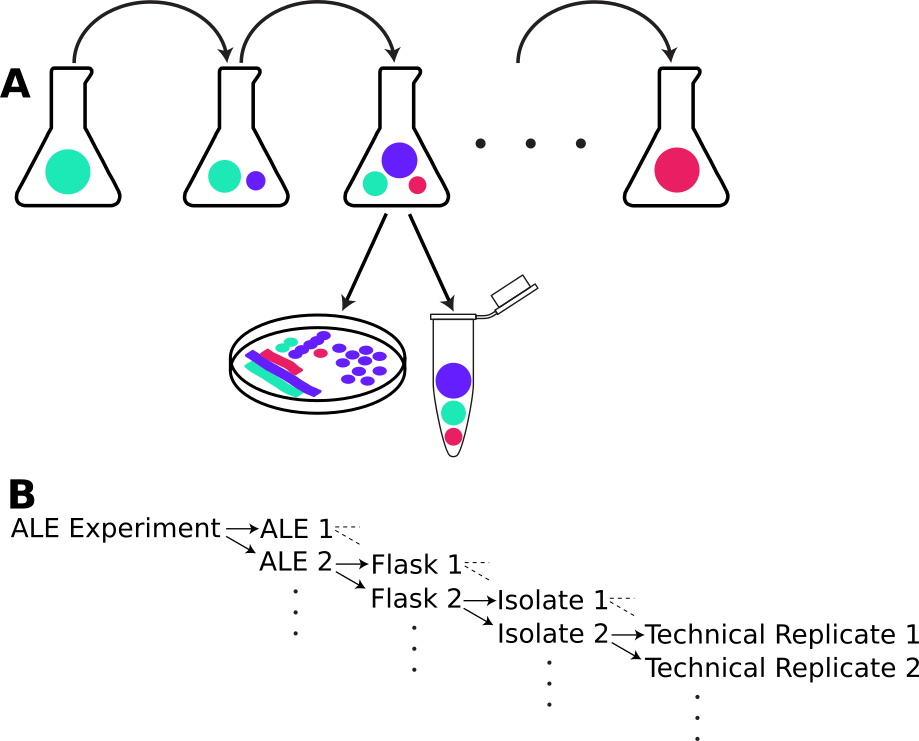
\includegraphics[width=1\textwidth]{ale_experiment_samples.png}
  \caption[An illustration of an ALE and its component organization]{\textbf{A} An illustration of an ALE from an ALE experiment where both a clonal and population sample are isolated from a midpoint flask. The petri dish illustrates the streaking out of a colony for capturing clonal samples. The Eppendorf tube illustrates a population sample of possible heterogeneous strains. \textbf{B} An illustration of how an ALE experiment can have many ALEs, flasks, isolates and technical replicates and how they are associated with each other.}
  \label{fig:ale_experiment_samples}
\end{figure}
The output of an ALE experiment are populations or clonal isolates which were derived from the original strain and additionally include the mutations in the cells according to the environmental stresses introduced in the ALE experiment. This output is then processed by additional foundational technologies leveraged with ALE: the DNA sequencer and mutation identifying software. The output sample to be analyzed is sequenced, typically by an Illumina platform, and resequenced primarily using the \textit{Breseq} computational pipeline \cite{breseq_paper}. Breseq's resequencing process aligns all of the DNA reads to a provided genome reference and reports single-nucleotide mutations, point insertions and deletions, large deletions, missing coverage and new junctions according to the differences between the aligned reads and the reference genome.

Generally, researchers compare the mutations from each ALE's endpoint samples to identify genomic regions with many alleles. If a researcher sequenced ALE midpoint or intermediate samples, an ALE's mutations can be organized in chronological order to identify mutations that fix. The mutations that are involved in multiple alleles of a genomic region or are shown to fix from starting or midpoint to endpoint samples are considered the \textit{key mutation} sets and are investigated for their possible fitness benefit according to the genomic region they affect.

% The ALE Analytics web platform leverages these fundamental technologies by importing the Breseq mutation predictions into a database and implementing a user web interface to enable the querying and curation of mutational trends. Currently, no other work has been published on the practical methodologies for analyzing ALE output; this thesis would be the first to publish on the concrete techniques and technologies used in interpreting ALE results en masse. This software pipeline and web platform will also accelerate the biological decision making necessary to leverage causal mutation for industrial and medical applications.

\subsection{ALE Machine}

ALE methodologies are becoming increasingly popular for their potential in revealing novel discoveries on evolution and designing organisms, though their wet lab execution is often labor intensive and requires significant run-time. To impose a balance on the required labor, many ALE experiments are designed to allow for approximately 24 hours between sessions. Executing manual ALE experiments often additionally restricts the possible experimental parameters according to the feasible amount of experiment monitoring. Current technologies in automation can be leveraged to automate many of the ALE processes, therefore alleviating these restrictions. Automation additionally can contribute to the consistency of the ALE experiments, better ensuring that artifacts in results are due to experimental conditions and not inconsistencies in experiment protocol execution. Finally, automation can enable the scale of an experiment to be greatly expanded at a much lower cost of effort to the experimentalists. This results in the potential for a larger amount of data to be generated on an ALE experiment, providing more resolution on the evolutions. These possible benefits have lead to the Systems Biology Research Group to develop an ALE automation platform, referred to as an \textit{ALE Machine} \cite{ryan_thesis}.

The ALE Machine eliminates many of the constraints that manual ALE experiments are subjected to, therefore enabling larger ALE experiments with more consistent data. These outcomes are a boon to those studying evolution and encourage experimentalists to further leverage ALE methodologies to explore the dynamics of evolution.


\section{Challenges}
% * <pphaneuf@eng.ucsd.edu> 2016-10-18T00:57:23.628Z:
% 
% NOTE: Be abstract in the description of the issues; the specific problems we were experience and our solution should be elaborated on later in the results of each aim with a case study.
% 
% ^.

The potential for more diverse and greater scale ALE experiments enabled by the ALE Machine's automation exacerbates existing challenges and introduces new challenges. The following is an itemization and description of each challenge considered for this thesis.

\subsection{Post-Processing Protocol}

Many tools exist for the quality control of sequencing data and the identification of mutations. Each tool comes with an inherent set of strengths and weaknesses. For the case of the SBRG's ALE operations, consistency in data quality is a primary priority that has been seen to vary between experiments. Additionally, a tool-set capable of identifying the majority of important genomic artifacts describing the difference between a reference genome and that of an evolved strain is necessary for the analysis of an ALE.

%More experiments translates to a higher probability of quality issues with any of the steps in the ALE experiment wet lab methodologies. Quality control measures are employed by most who work with sequencing data, though the process and tool-set employed by each individual may vary. For our ALE experiment post-processing, a quality control process needed to be established to ensure consistent ALE experiment result quality.

\subsection{Experiment Data Consolidation Effort}

As the scale of an ALE experiment grows, so too does the effort necessary to curate the data of the experiment's samples into a report that describes the ALE experiment's mutation lineages. These manual curations are additionally prone to human error, which is more likely to occur with larger experiments.

\subsection{Result Accessibility}

ALE experiments often involve multiple experimentalists and collaborators. The input of many collaborators may be necessary to fully capture and understand the results of an experiment. These collaborators may be locally or remotely located. The logistics of sharing results is often challenging between local collaborators and more problematic between remote collaborators. This is especially true when comparing multiple experiment results from both current and past ALE experiments.

\subsection{Experiment Analysis Effort, Consistency and Accuracy}

The issues of data consolidation with larger scale experiments also manifest with the analysis of the experiment results. The key mutation analysis of experiments may be inconsistent between investigators. Key mutations may be excluded from the analysis of the results depending on the amount of experience of an ALE experimentalist. Different methods of reporting experiment results may be used between experimentalists, therefore making the comparison of different ALE experiments more difficult.


\section{Specific Aims}

We have defined a specific set of aims that would lead to solutions to these challenges. The aims are as follows:
\subsection{Aim 1: Establish a Post-Processing Protocol}
To ensure the consistency of quality and format of ALE experiment data, we aim to establish a post-processing protocol. This pipeline will take as input ALE experiment sample sequence data and output reports on each sample's mutation set with regards to a reference genome. Before the mutation reports are generated, reports on the sequencing data quality are generated and inspected; if necessary, measures will be taken to improve the quality of the sequencing data.
\subsection{Aim 2: Automate ALE Experiment Data Consolidation and Accessible Report Generation}
To reduce the effort in generating consistent ALE experiment mutation lineage reports that combine all appropriate ALE experiment samples, we must develop software to automate the parsing and databasing of ALE experiment mutation data. This database will then be leveraged by a reporting application that will produce mutation lineage reports. To address the challenge of results accessibility, the application used to generate ALE experiment reports will be developed as a web application which can be made accessible to collaborators over the web. This application will be able to present all available ALE experiment mutation and results reports.
\subsection{Aim 3: Automate Common ALE Experiment Analysis}
% * <pphaneuf@eng.ucsd.edu> 2016-10-27T16:34:32.855Z:
%
% TODO: Speak towards the fact that we're handling issues with accuracy, consistency and the ability to automatically amend results with new protocols.
%
% ^.
The common methods of identifying an ALE experiment's key mutations will be defined and automated; their results will be presented by the reporting features alongside the mutation lineage reports.

%The most immediate significant impact will be with building a software platform that will automate the organization and report generation for ALE experiments. SBRG researchers can spend weeks manually organizing mutational data in order to identify mutations \textit{significant} to the evolutions of a strain in an ALE experiment. This manual investigation is also prone to human error, where researchers may overlook significant mutations. The resolution on the mutational information from an ALE experiment is also limited by the time cost for manually curating mutational lineages; automating this curation allows for researchers to incorporate more sample sequencing data into their investigation to establish more resolution on mutational trends in their experimental evolutions.

%The final impact is how the work generated with this thesis has the potential to aid in novel discoveries. We leverage the resulting ALE mutation database to develop features that enable researchers to investigate mutational artifacts and trends across all current ALE mutation data.


\chapter{Aim 1: Establish a Post-Processing Pipeline}

%"execute research on past resequencing performance data to empirically create a set of performance metrics tailored to our instrumentation and process according to our expected outcomes. With these performance metrics, we’ve established a quality control processes for our sequencing data, ensuring that we are not incorporating poor data into the ALE Analytics web platform."

\begin{figure}[h!]
  \centering
  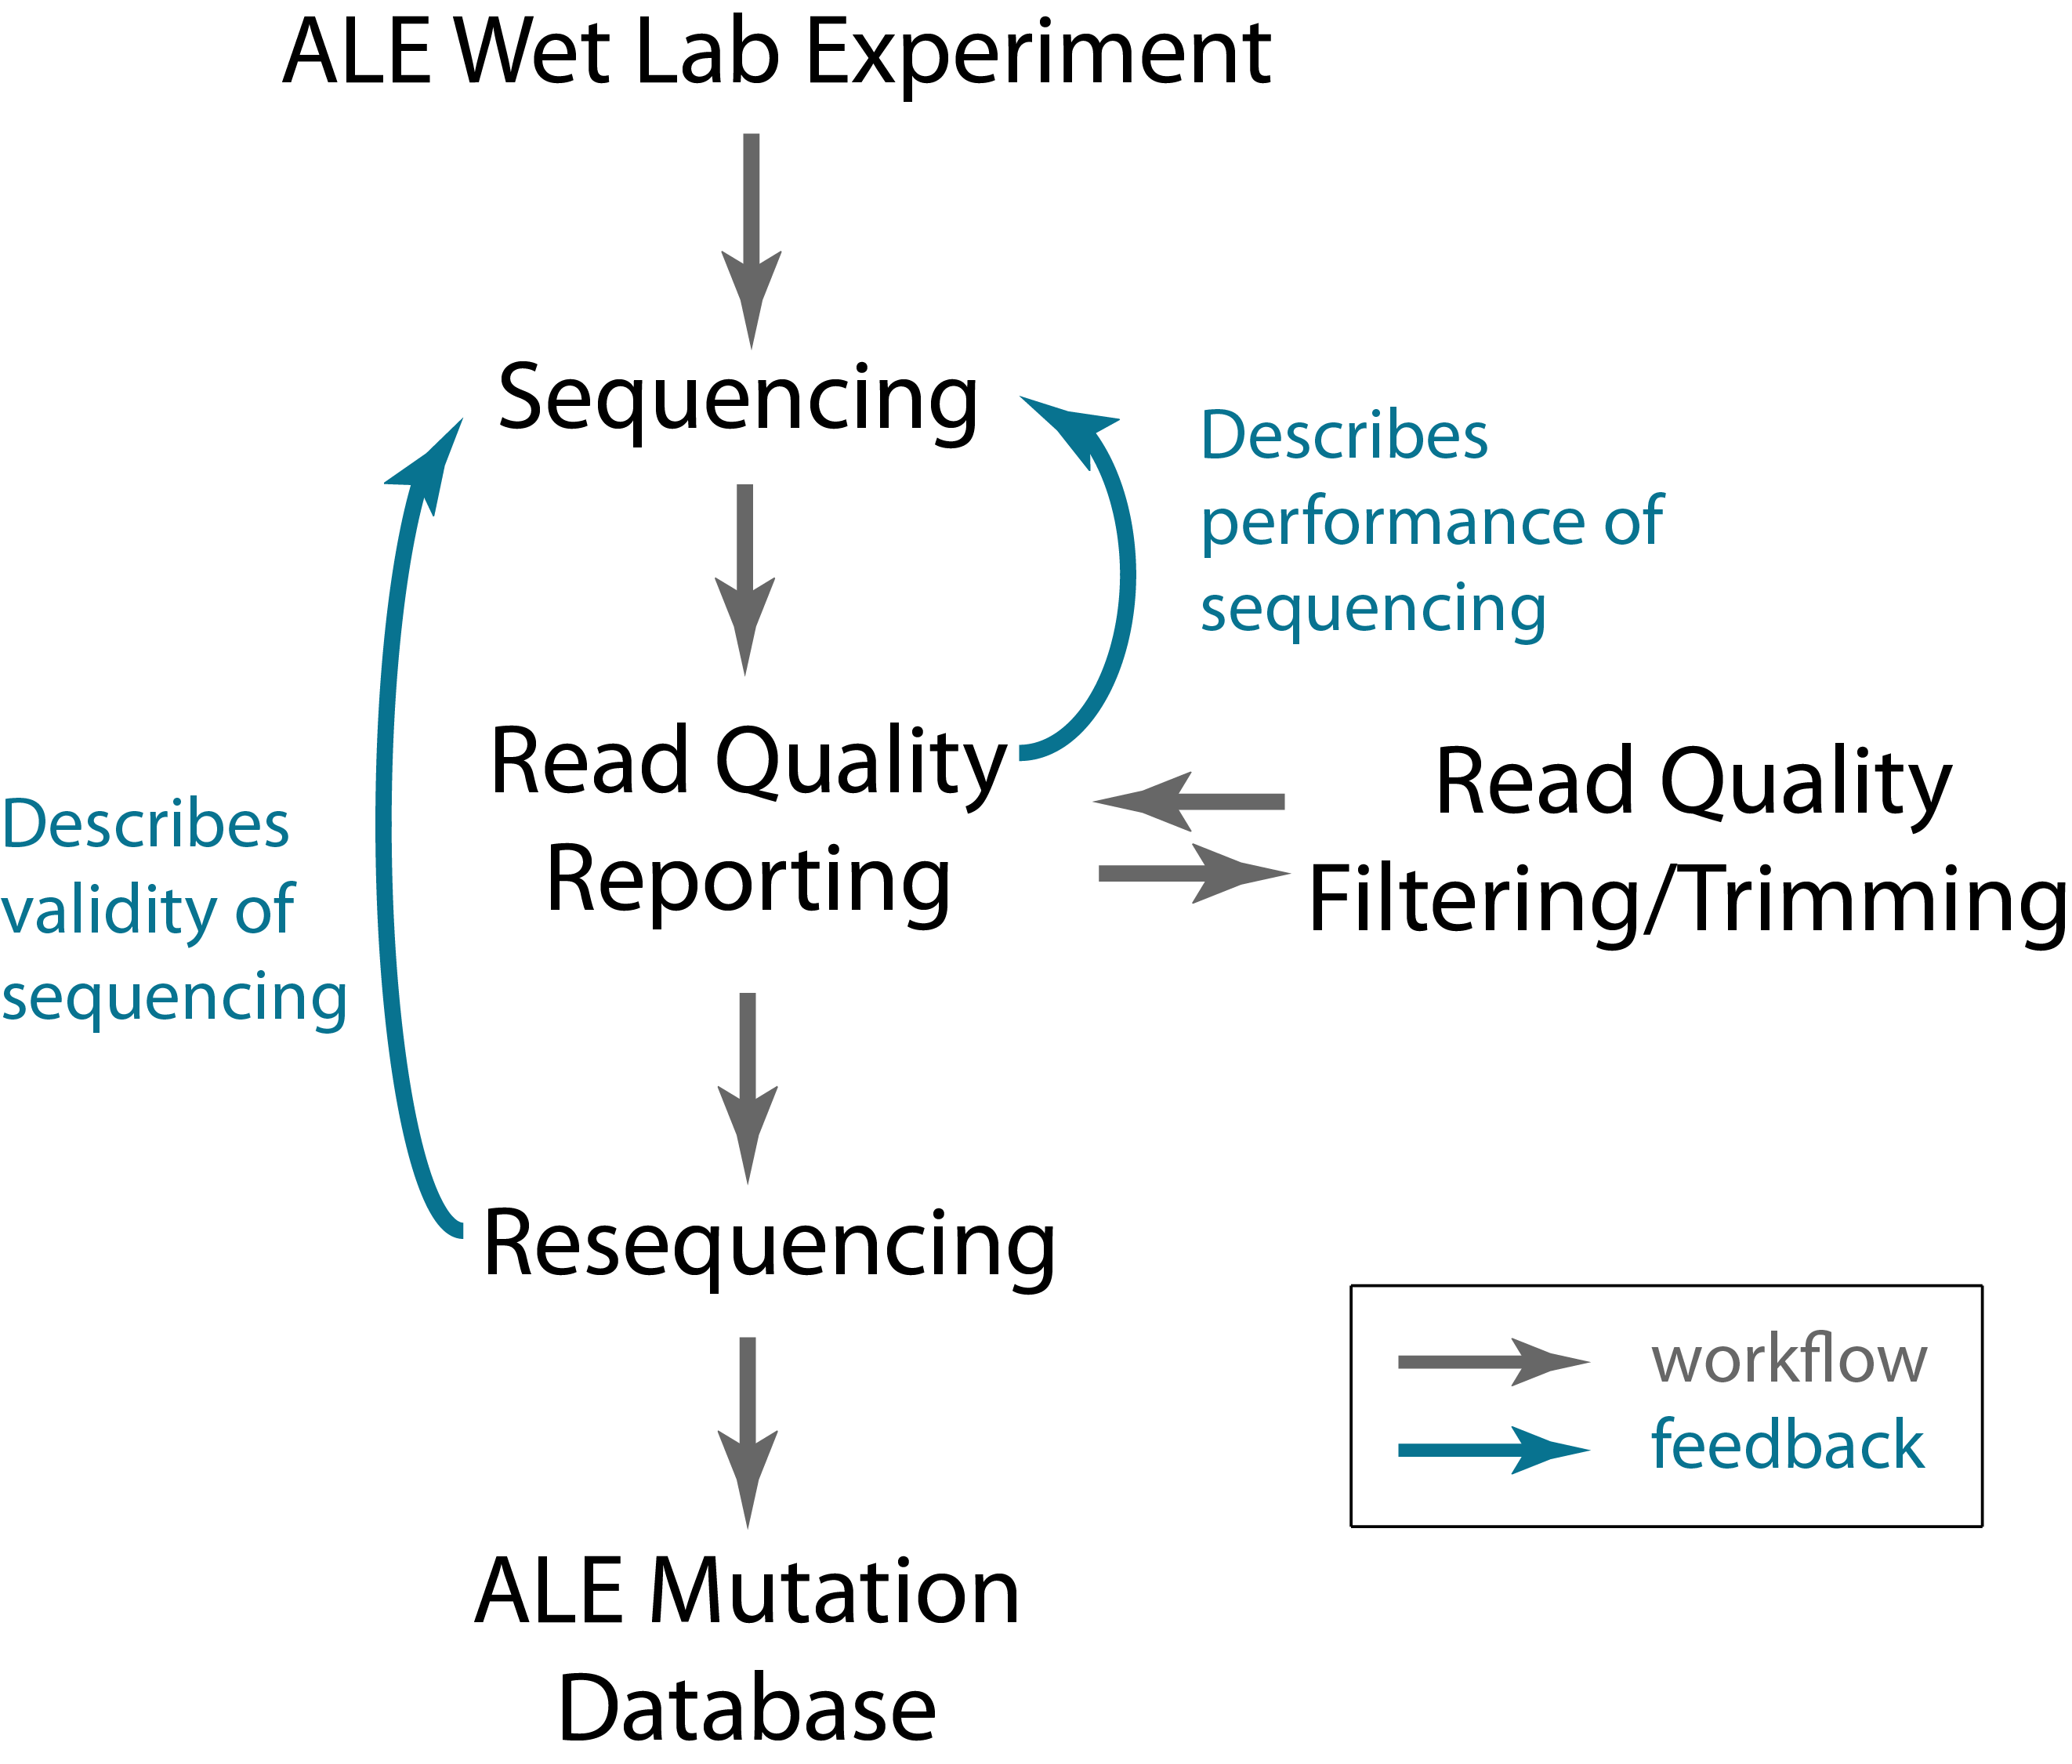
\includegraphics[width=0.7\textwidth]{post-processing-protocol.png}
  \caption[An illustration of the ALE sample post-processing protocol, software pipeline and feedback targets. ]{The term \textit{resequencing} describes the alignment and variant identification process with given reads relative to a reference genome.}
  \label{fig:post_processing_protocol}
\end{figure}
We have established a post-processing protocol for the quality control of the sequencing data and to capture each sample's mutations. The protocol uses the following software: \textit{FastQC} \cite{Andrew} for sequenced reads quality analysis, the \textit{FASTX-Toolkit} \cite{FASTX-Toolkit} for trimming sequenced reads, and Breseq \cite{breseq_paper} to align reads to a reference genome and identify mutations relative to a reference genome.

% * <pphaneuf@eng.ucsd.edu> 2016-11-21T16:29:53.433Z:
%
% TODO: could reference the following paper to describe the biasing of bases: https://www.ncbi.nlm.nih.gov/pmc/articles/PMC4351865/
%
% ^.

The protocol first requires that the reads for all sequenced ALE samples are inspected for their \textit{per base sequence quality} and \textit{per base sequence content} using FastQC. The per base sequence quality report presents the cumulative quality score of the bases in specific read positions as having good, reasonable or bad quality. From these results, we can understand which 3' and 5' read end positions have the lowest cumulative quality and trim these positions out using the FASTX-Toolkit. We additionally inspect the per base sequence content for any abnormalities such as the biasing for particular bases in specific positions. In a random set of sequenced reads, you would expect that each read position has approximately equal counts of each base, though in our more recent samples, we often experience a biasing of base types in the first 17 positions and the final 25 positions of each read. At this point, we additionally noticed that many alignment artifacts being identified as mutations in our subsequent variant calling were located in these read regions. This base type biasing is likely due to the sequencing library preparation chemistry that inherits an intrinsic DNA fragmentation sequence bias \cite{Head2014}. Though this bias does occur, it should theoretically not result in inappropriate base calling. Even so, trimming these biased regions out of our reads has lead to less mutation calling due to sporadic non-consensus bases. The process of quality inspection and trimming may iterate multiple times before moving on. Once the reads report acceptable quality, Breseq is used to align each sample's reads to a reference genome and identify mutations. In addition to mutations, Breseq reports return the alignment statistics of \textit{mean coverage} and \textit{mapped read} count. In combination with the amount of \textit{unassigned missing coverage} evidence, regions where no reads could be aligned to the reference, these statistics are used to evaluate the alignment performance, where we compare each statistic and unassigned missing coverage artifact count to an empirically derived threshold. If the mean coverage or mapped read values fall below our thresholds or the unassigned missing coverage artifact count exceeds our thresholds, we consider the sequencing library of the sample they belong to as potentially problematic in our analysis of the evolution and may again sequence the sample or discard them from the analysis.

Besides the actual generation of mutation data, the key functionality of our post-processing protocol is the stage dependent feedback provided. This feedback offers the opportunity for experimental protocol and data acquisition refinement that can be acted on by the many individuals involved in the sample preparation and processing pipeline.

% * <pphaneuf@eng.ucsd.edu> 2016-10-18T02:58:09.248Z:
%
% TODO: Give example of how this protocol increased our results quality and consistency.
%
% ^ <pphaneuf@eng.ucsd.edu> 2016-10-18T02:59:49.020Z:
%
% Example of results quality increase was given in an ALE Happy Hour meeting a while back, though this includes data from projects that aren't yet public.
%

\chapter{Aim 2: Automate ALE Experiment Data Consolidation and Generate Accessible Reports}

% * <pphaneuf@eng.ucsd.edu> 2016-10-13T18:05:59.630Z:
%
% Should I GENERALLY describe the schema of the ALE mutation database?
%
% ^.

%The products of this thesis have been primarily driven by the need to consolidate and report on large amounts of ALE experimental data in such a way to describe the quality of the sample sequencing, adaptive mutations in evolved strains, the context of mutations via their meta data (i.e., culturing environments, strain properties), and related mutations found in other experiments housed in an ALE mutation database. We have done so by leveraging a full stack of technologies that enable the parsing and databasing of experiment mutation and meta data, the execution of automated analysis on said data and the generation of web accessible reports.

% The process of accumulating all ALE experiment mutation data into a query-able uniform resource has lead us to employ current databasing technologies. The \textit{ALE mutation database} is the product of this process, containing and organizing all ALE experiment mutations and meta data ultimately employed by the other products of this thesis.

The products of this thesis have been primarily driven by the need to consolidate and report on large amounts of ALE data in such a way as to describe adaptive mutations in evolved strains. We have done so by leveraging a full stack of industry standard technologies that enable the parsing and databasing of experiment data and the generation of reports on said data.
\begin{figure}[H]
  \centering
  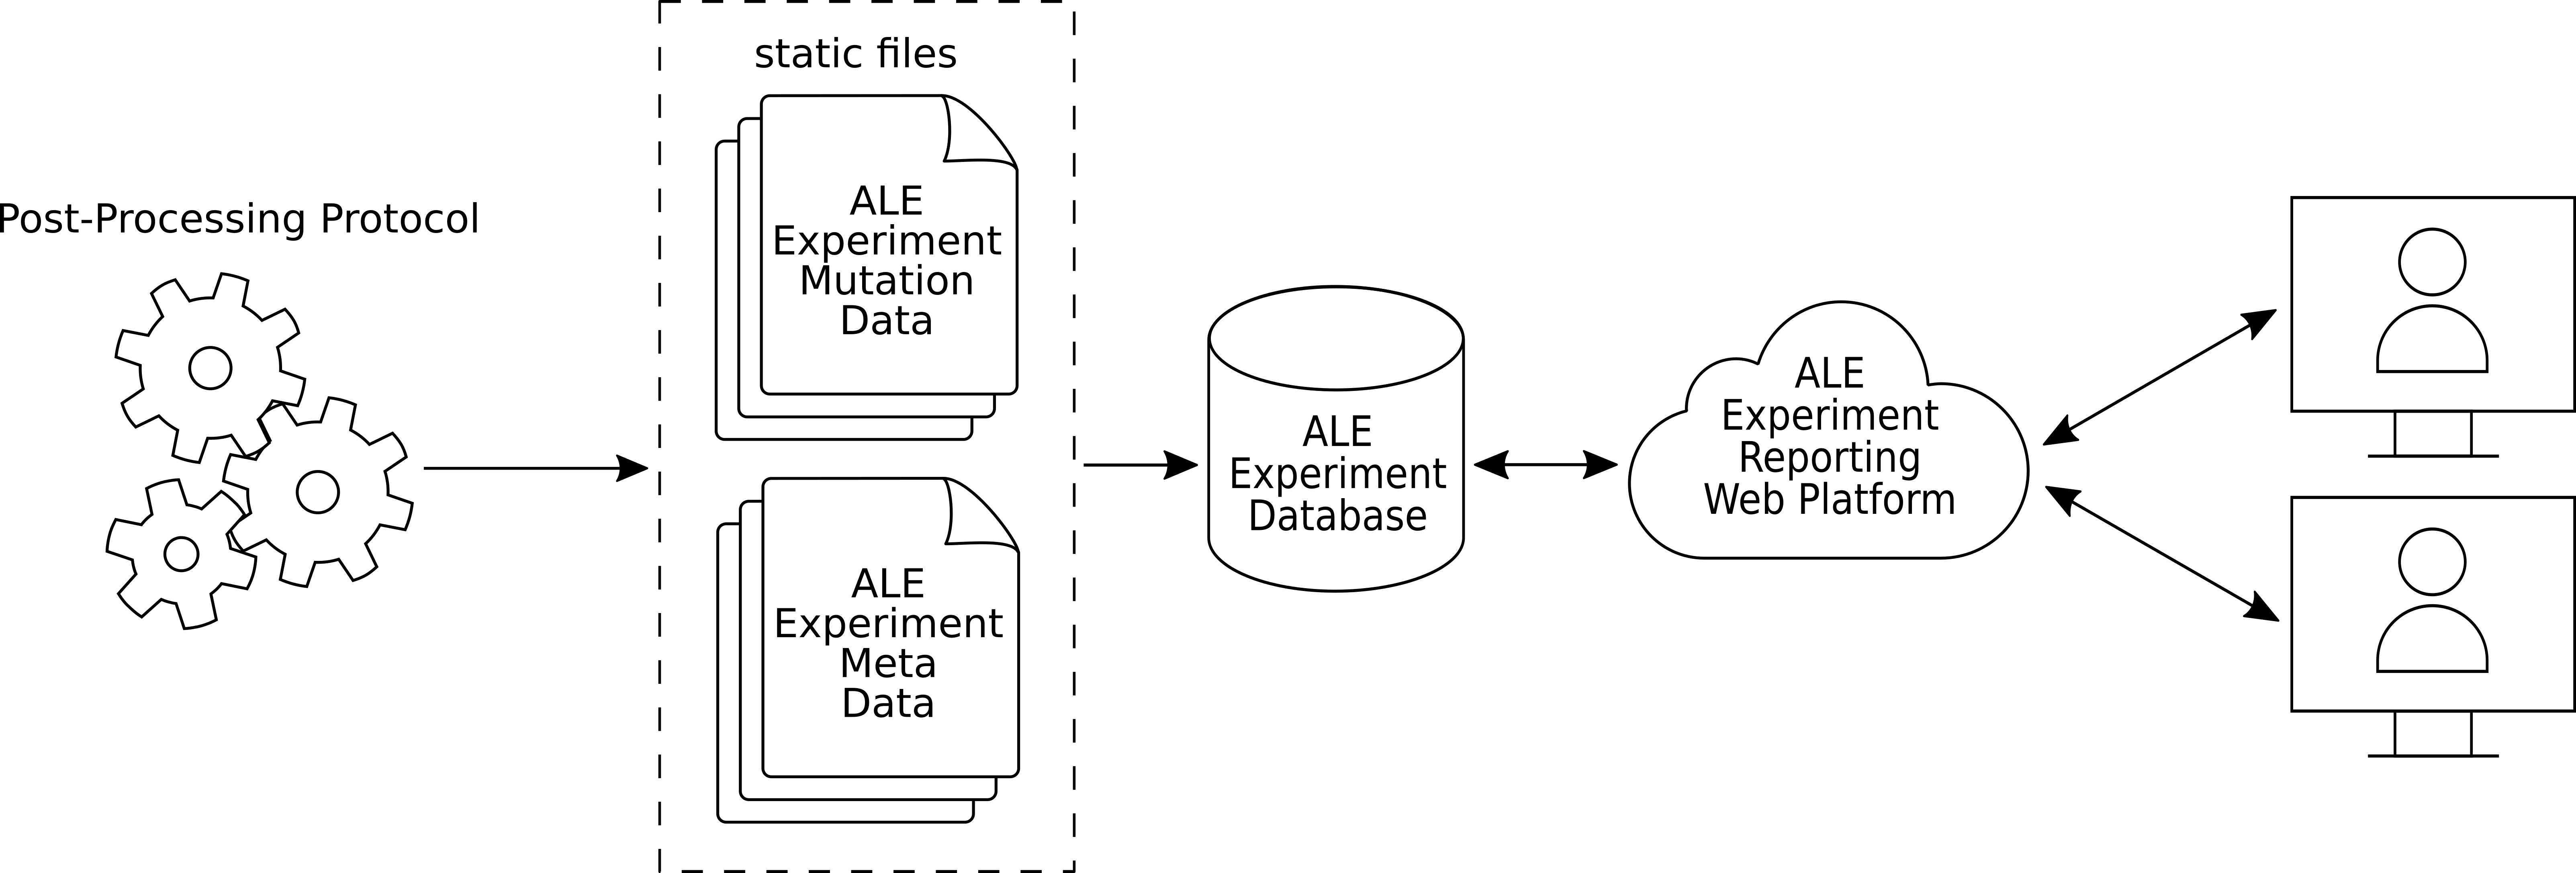
\includegraphics[width=1\textwidth]{simple_deployment_diagram.png}
  \caption{An illustration of the flow of ALE experiment data to the deployment of result report generation for end users.}
  \label{fig:simple_deployment_diagram}
\end{figure}

The automation manifests as the programmatic parsing of the mutation reports generated by Breseq for all ALE experiment samples and with the mutational data subsequently loaded into an ALE mutation database. During the initiation of an ALE experiment, experimentalists generate meta data which can be additionally parsed and uploaded to the ALE mutation database by the automated parsing of ALE experiment data. This process consolidates all experiment mutation data and meta data into one resource. This database is used for all ALE experiments and therefore has resulted in all available ALE experiments being consolidated into one database, enabling further cross-experiment analysis.

The ALE mutation database is leveraged by a web application to automate the generation of reports for each ALE experiment that describe the mutational lineages of their ALEs. This application is deployed on the web, allowing for ubiquitous accessibility to ALE experiment reports for all experimentalists and collaborators. We have named this web application ALE Analytics.

\section{ALE Analytics Web Platform}

% * <pphaneuf@eng.ucsd.edu> 2016-10-21T00:48:08.332Z:
%
% Example of consistency results can be shown with the means of reporting on ALE experiment mutation results from the 4 ALE papers and how they are missing information in the papers and the full data provided in the supplementary material isn't perfect.
%
% ^.

The ALE Analytics web platform enables and automates much of the analysis necessary for interpreting ALE experiment mutational data. For this thesis, we primarily describe the automated mutation analysis and reporting features, though this platform additionally includes ALE \textit{mutation filtering},  \textit{mutation search}, \textit{ALE experiment export} to CSV, \textit{ALE experiment comparison}, sample sequencing data alignment \textit{quality statistics} and \textit{mutation database overview}. The fundamental focus of the ALE Analytics web platform is report generation. Each ALE experiment can be described as a series of samples which contain both new mutations and mutations from ancestors relative to a reference genome. Ordering the samples as columns from earliest to latest in an ALE, where each row describes the manifestation of a specific mutation among samples, can serve as a visualization to grant intuition on mutational trends. The occurrence of a mutation in a sample is annotated as a value between 0 and 1 within the cell of a mutation row for the sample. The annotated value represents the estimated frequency of this mutation among the sample population \cite{breseq_paper}. Among the many mutations that manifest within an ALE experiment, mutation rows that describe the alleles of a gene in the ALE experiment will cluster together due to the sorting of mutations according to their positions on the genome. Due to the chronological sorting of the sample columns per ALE, a mutation that fixes across samples will manifest as a sequence of cells in a mutation row annotated with the manifestation of that mutation. These patterns are obvious to an observer and serve well to describe the mutation trends in an ALE experiment.

\begin{figure}[H]
  \centering
  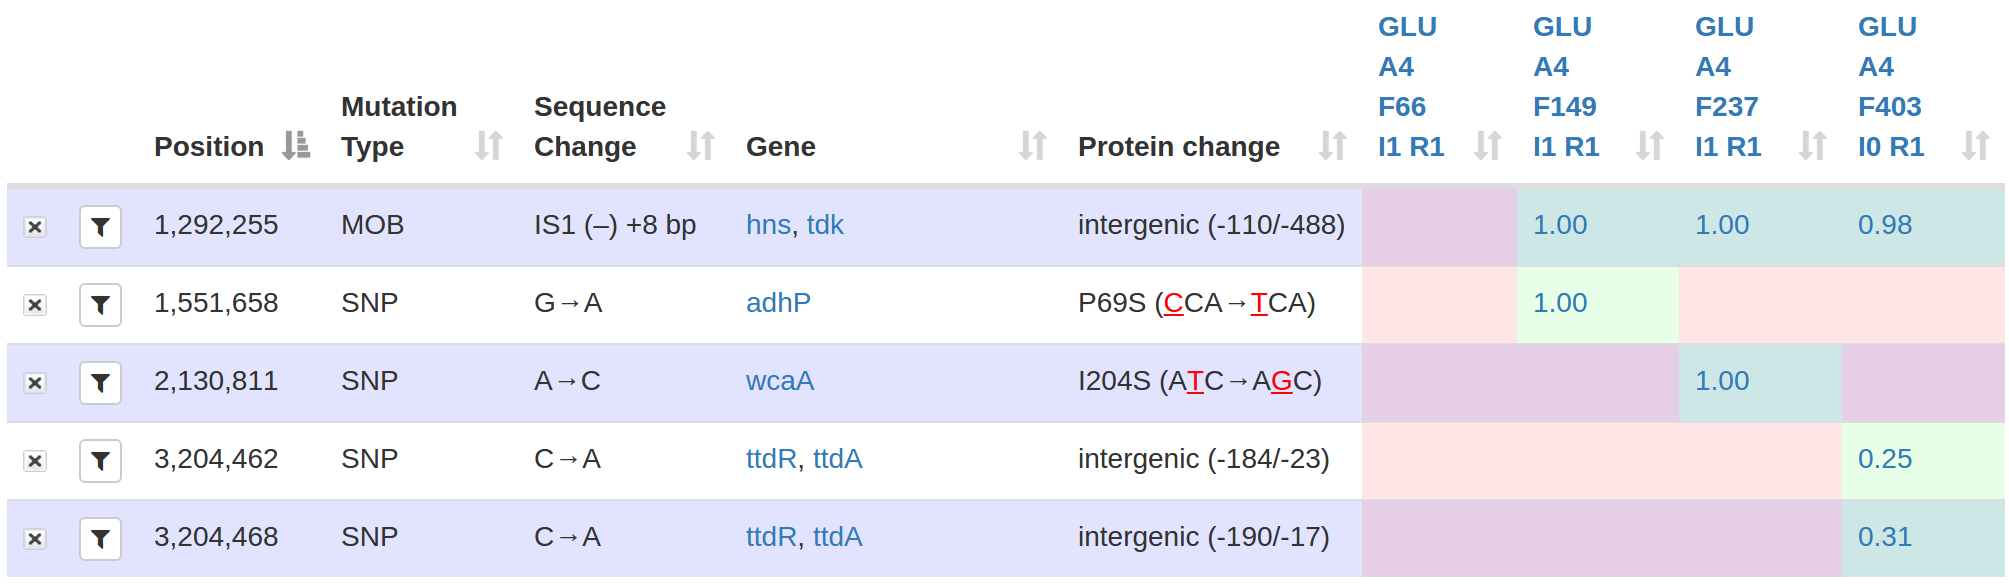
\includegraphics[width=1\textwidth]{mutation_lineage_report.png}
  \caption{Illustration of a mutation lineage report. The \textit{hns, tdk} intergenic mutation and a \textit{corA} mutation can be seen to fix in samples over time. The multiple mutation rows describing the \textit{corA} alleles cluster together.}
  \label{fig:mutation_lineage_report}
\end{figure}

% * <pphaneuf@eng.ucsd.edu> 2016-10-20T03:12:25.010Z:
%
% TODO:  ensure that the following paragraph is appropriate and shouldn't be placed elsewhere. It could be used to describe the significance of the platform, which is appropriate for this section.
%
% ^.
Before the ALE Analytics platform was deployed for use, experimentalists would work to identify ALE experiment \textit{key mutations} by manually annotating all ALE experiment sample mutations within a spreadsheet and investigate for significant mutation patterns. The task of manually annotating mutations proved to be time consuming and error-prone, causing delay of ALE experiment result interpretation. This initial bottleneck in the post-processing of ALE experiment results lead to the efforts that began the ALE Analytics project. The time cost of this manual curation additionally set an implicit limit on how many samples experimentalists were willing to sequence and process into their output data set, therefore potentially limiting the resolution on an ALE experiment's mutational trends. Additionally, the type of sample obtained from a flask was limited by the cost of manual curation according to the amount of mutations annotated per sample, where population samples can include an order of magnitude more mutations than clonal samples; this can therefore cause an experimentalist to limit the inclusion of population samples into an ALE experiment's output data set. The primary function of the ALE Analytics platform is to automate the annotation and reporting of all ALE experiment sample mutations in a single location with a uniform format. This automated functionality enables experimentalists to more quickly interpret results and include more sequenced samples into their mutation set, without fear of the effort necessary in processing and consolidating their experiment's mutational data. Alongside the ALE Machine, ALE Analytics further enables more resolution on evolution. This automation may additionally result in more consistent reporting and accurate results since it removes the potential for human error in data processing, consolidation and report generation.

Since August 2015, the ALE Analytics web application has deployed a production version for experimentalists and collaborators to use in the analysis of their ALE experiments. Though we have many development versions that are launched and shutdown for testing and demonstrating new features to target audience, our production version of ALE Analytics has constant uptime and is available online for access by local and remote experimentalists and collaborators. To end-users, ALE Analytics represents a web platform and database of experimental evolution results that is ubiquitously available and ever growing in features and content.

\begin{figure}[H]
  \centering
  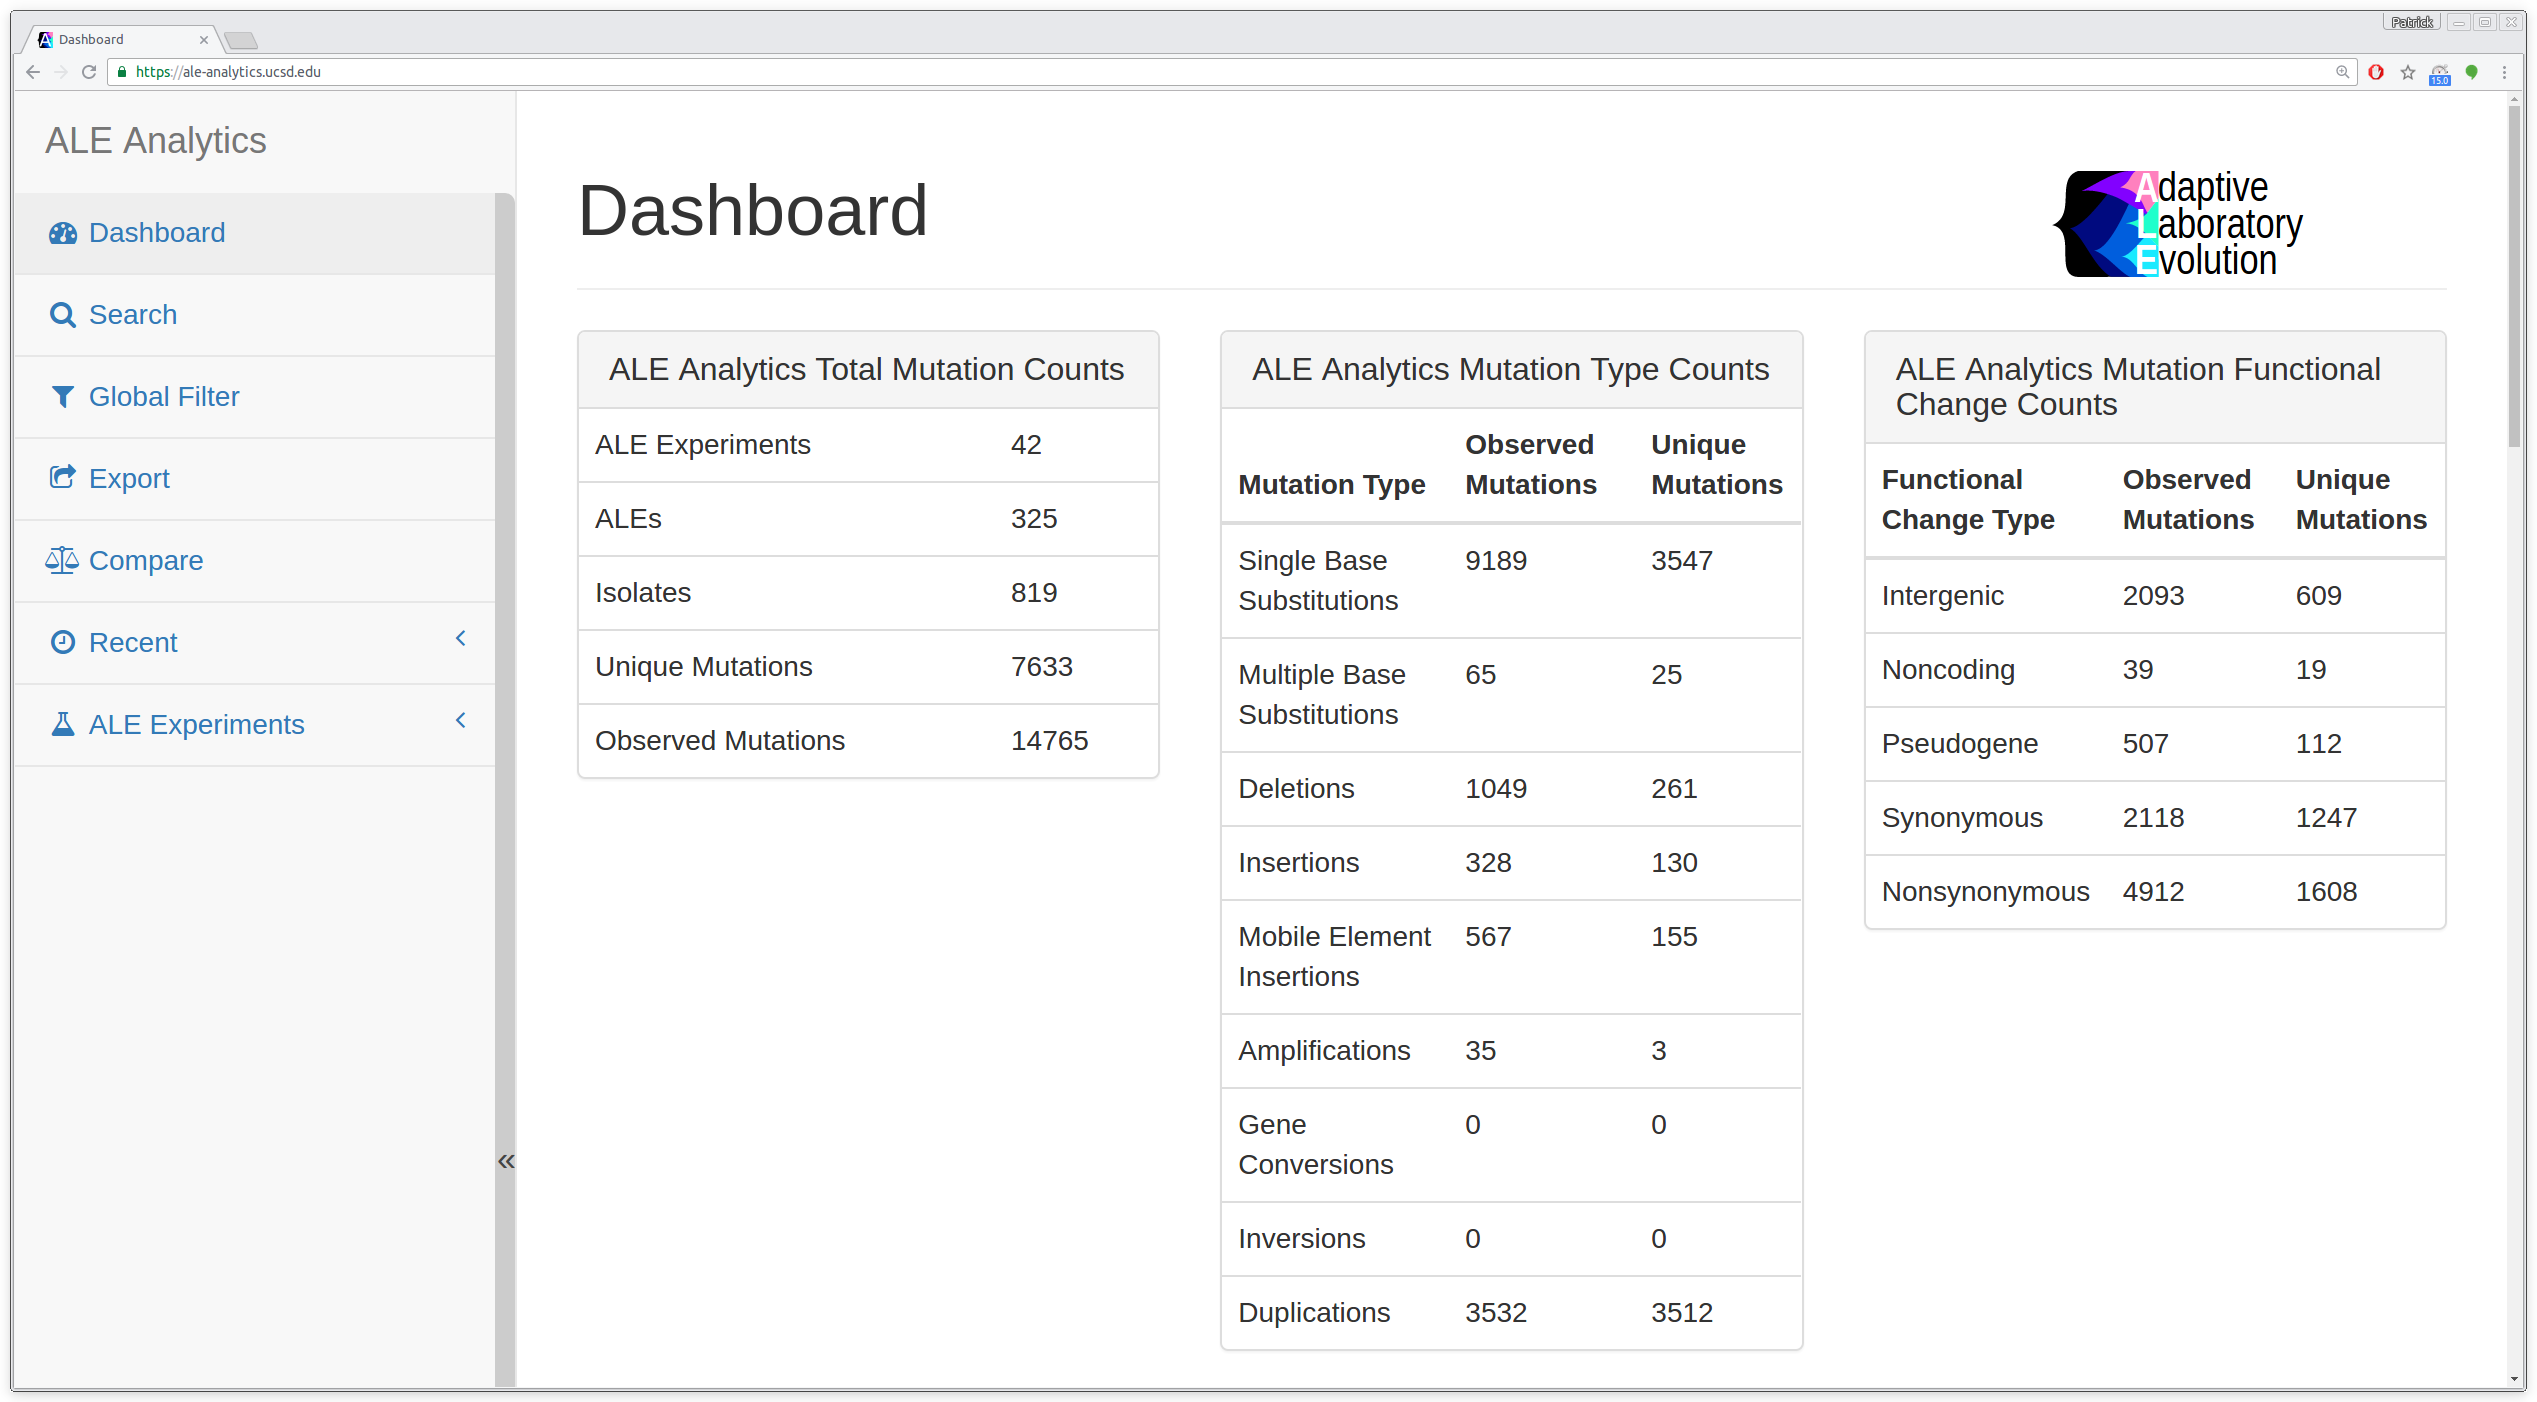
\includegraphics[width=1\textwidth]{dashboard_screenshot.png}
  \caption{Screenshot of the ALE Analytics production version dashboard containing counts of significant ALE mutation database details.}
  \label{fig:dashboard_screenshot}
\end{figure}

The current production deployment of ALE Analytics contains 14,765 observed mutations and 7,633 unique mutations. These mutations are housed in 42 separate ALE experiments with a total of 325 ALEs and 819 isolates or samples. This large volume of mutations and samples is evidence to how the the automation of consolidating ALE experiment data has been leveraged to create a substantial resource on experimental evolutions. Being that ALE Analytics is being leveraged in investigating current experiments, full access hasn't yet been made available to the public. Our intent is to ultimately make public on ALE Analytics the results of the ALE experiments that have been published.

\clearpage
I would like to acknowledge the work accomplished by Dr. Ali Ebrahim, Dr. Ryan LaCroix, Kaiwen Zhang and Dylan Skola for their early prototyping on what we now know as ALE Analytics.

I would like to acknowledge Dennis Gosting for his work in consolidating ALE experiment data into the ALE mutation database.
% * <pphaneuf@eng.ucsd.edu> 2016-10-20T17:06:22.581Z:
% 
% TODO: could insert figure here that describes:
% 1) more ALEs.
% 2) more samples per ALE
% 3) population samples rather than clonal samples
% 
% ^.
\chapter{Aim 3: Automate Common ALE Experiment Analysis}

Using the ALE Analytics mutation reporting mechanism, we have implemented features that automate the finding and reporting of mutations which describe significant mutational patterns within an ALE experiment. These features describe the significant mutation patterns as \textit{enrichment} and \textit{fixed} mutations. The methodologies encapsulated in the enrichment and fixed mutation analysis are those which have been developed to manually identify key mutations within the results of published ALE experiments (\cite{10.1371/journal.pgen.1001186}, \cite{pmid25015645}, \cite{pmid26964043}, \cite{pmid25304508}) and are therefore considered common ALE experiment key mutation analysis. As with the manual consolidation of ALE experiment mutational data, the analysis of key mutations can be prone to human error, inconsistent between researchers and time consuming. The automation of these common analyses will contribute to more accurate results, more consistent analysis and the shortening of turnaround time from ALE experiment execution to results interpretation.

% * <pphaneuf@eng.ucsd.edu> 2016-08-13T23:12:01.842Z:
%
% identifying mutations in the same gene/region across replicate experiments Mutation persists across many samples (fixation); Specific mutation no longer detected, but another mutation in the same gene was identified; Found at multiple points of clonal analysis -GLU paper
%
% ^.

\section{Enrichment Mutation Analysis}

% * <pphaneuf@eng.ucsd.edu> 2016-08-13T23:19:05.611Z:
%
% "These key mutations were straightforward to identify as the given genetic regions were reproducibly mutated across multiple ALE experiments." -GLU
%
% ^.

% * <pphaneuf@eng.ucsd.edu> 2016-08-14T21:56:31.904Z:
%
% "Several genes and genetic regions were identified that contained mutations across many of the independent ALE experiments, implying causality." -GLU paper
%
% ^.

% * <pphaneuf@eng.ucsd.edu> 2016-08-13T21:53:16.311Z:
%
% "This mutational recurrence pointed to the key genetic targets underlying the evolved fitness increase."
%
% ^.

Early ALE experiments only sequenced ALE endpoint samples. Key mutations were identified as those involved in the following two cases. If a mutation manifested in more than one sample, it signified that this mutation was likely correlated to the dominant phenotype. If a genomic region was mutated via different mutations across multiple samples, it was hypothesized that simply perturbing the gene may have rendered a benefit to the phenotype. Considering that these circumstances all involve populations with the same mutated genomic region, we can also consider a single sample with multiple alleles of the same region to represent multiple populations which benefit from this region's perturbation. The identification of these cases can be accomplished by finding genomic regions within an ALE experiment that have more than one observed mutation; we consider these enriched genomic regions and their mutations as enrichment key mutations. Previous to ALE Analytics, this analysis was accomplished as additional steps in manually curating the ALE experiment's mutation report such that mutations affecting the same genomic region would cluster together within a matrix of mutations and their samples. The \textit{enrichment mutation} analysis automates this approach and reports the mutations in the same mutation reporting format given in Figure \ref{fig:mutation_lineage_report}.

\begin{figure}[H]
  \centering
  
\includegraphics[width=0.3\textwidth]{enrichment_mutation_flowchart.png}
  \caption{Enrichment mutation analysis flowchart}
\end{figure}

\section{Fixed Mutation Analysis}

A fixed mutation is one in which a mutation manifests in an ALE's midpoint, or intermediate sample, and is propagated to all following samples in the ALE. Fixed mutations are the strongest indicators of key mutations. This analysis is possible if an ALE experiment includes midpoint samples, so as to provide for the possibility of more than one data point per mutation. Previous to ALE Analytics, the identification of Fixed mutations was accomplished as an additional curation step in results reporting by manually organizing mutations according to their ALE's sample chronology and subsequently identifying mutations that emerge in a midpoint and manifest in all remaining ALE samples. The \textit{fixed mutation} analysis automates this approach and reports the mutations in the same mutation reporting format given in Figure \ref{fig:mutation_lineage_report}.
\begin{figure}[H]
  \centering
  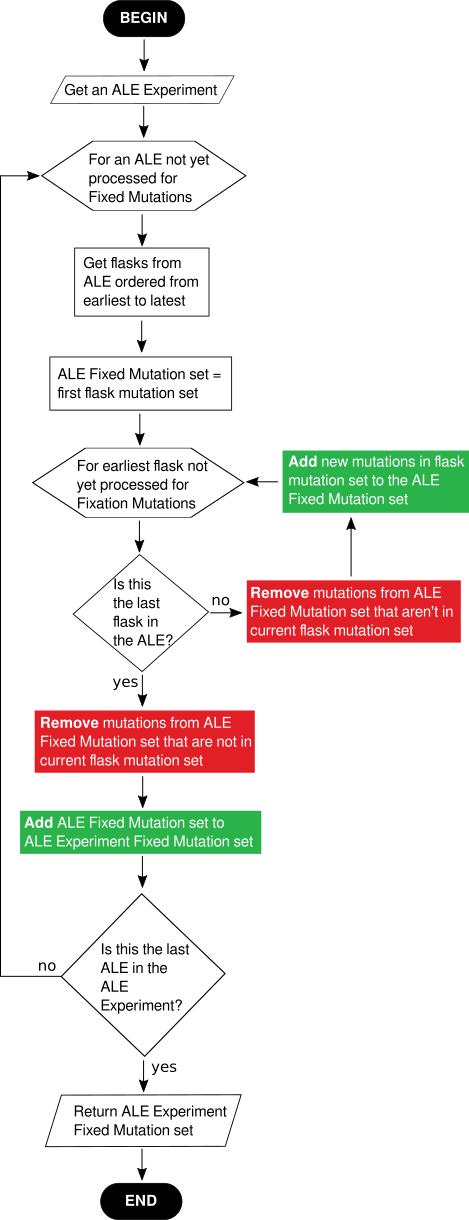
\includegraphics[width=0.50\textwidth]{fixed_mutation_flowchart.png}
  \caption{Fixed mutation analysis flowchart}
\end{figure}
Ideally, fixed mutations should have frequencies equal to or larger than their preceding occurrences within an ALE. This trend demonstrates the most obvious key mutations within a ALE experiment. The fixed mutation analysis has a filtering option that results in only those fixed mutations with equal-to or ascending population frequency trends to be returned. This feature is referred to as the \textit{ascending frequency} fixed mutation analysis and reports these mutations in the same mutation report format given in Figure \ref{fig:mutation_lineage_report}.
\begin{figure}[H]
  \centering
  
\includegraphics[width=0.4\textwidth]{ascending_freq_fixation_mutation_filter_flowchart.png}
  \caption{Ascending frequency fixed mutation analysis flowchart}
\end{figure}
\section{Results}
% * <pphaneuf@eng.ucsd.edu> 2016-10-11T02:35:45.973Z:
%
% TODO: We also investigate any new key mutations by ALE Analytics and potentially corroborate these new findings with the published materials.
%
% ^.

To ensure that our automated key mutation analysis returns key mutations based on published criteria, we evaluate the automated analysis results against those found in ALE experiments published by the SBRG. The automated analysis key mutations are generated by processing the sample reads available from these published ALE experiments through the post-processing protocol, ALE Analytics platform and key mutation automated analysis. Intuitively, our task can be described as finding all of the key mutations within the complete set of mutations in an ALE experiment and comparing the set for equality against the published key mutation set of the same experiment. The post-processing protocol will be configured to reproduce, as well as possible, the mutation set used by the authors in defining the published key mutations by using the same reference genome and Breseq version. This does not guarantee that the mutation set produced will be identical to those used by the authors and therefore introduces the issue of having different starting conditions between key mutation analysis.

% * <pphaneuf@eng.ucsd.edu> 2016-10-22T17:45:47.614Z:
%
% Talk towards what are the probabilistic circumstances that cause the potential for different mutations to be called from those used in the papers to identify key mutations.
%
% ^.
We find a more practical comparison for our automated key mutation analysis evaluation to avoid issues due to possible different ALE experiment mutation sets between the published material and those generated by the post-processing protocol. Clarification of gene function is a primary result in ALE experiments. Organisms studied in ALE experiments are selected for their phenotype which is derived from their genotype. For ALE experiments, the areas of highest interest in a genotype are those genomic regions perturbed by mutations. With ALE experiment mutation sets, experimentalists investigate the known functions of the perturbed genomic regions along with the phenotypic results of the perturbation and infer additional functions of genomic regions. We can therefore reason that a better evaluation between the results of the published ALE experiments and the ALE Analytics automated analysis is a comparison of the genomic regions found to be perturbed by key mutations. We discuss any false positives and false negatives and determine why they manifest and what can be implemented to handle their specific cases. The following is the set of publications that we use in our evaluation and their ALE experiment names:
\begin{itemize}
\item \textbf{The PGI ALE experiment}: \textit{Genetic Basis of Growth Adaptation of Escherichia coli after Deletion of pgi, a Major Metabolic Gene.} \cite{10.1371/journal.pgen.1001186}
\item \textbf{The 42C ALE experiment}: \textit{Evolution of Escherichia coli to 42 °C and Subsequent Genetic Engineering Reveals Adaptive Mechanisms and Novel Mutations. Molecular Biology and Evolution.} \cite{pmid25015645}
\item \textbf{The \textit{13C }ALE experiment}: \textit{Evolution of E. coli on [U-13C]Glucose Reveals a Negligible Isotopic Influence on Metabolism and Physiology.} \cite{pmid26964043}
\item \textbf{The \textit{GLU }ALE experiment}: \textit{Use of Adaptive Laboratory Evolution To Discover Key Mutations Enabling Rapid Growth of Escherichia coli K-12 MG1655 on Glucose Minimal Medium.} \cite{pmid25304508}
\end{itemize}
\section{Evaluation}
In this section we describe our approach to formally evaluating the performance of our key mutation automate analysis. The task of finding key mutations is a binary classification problem, where a mutation is or is not a key mutation. To accomplish binary classification on a set of mutations, we have defined a set of features that describe how a mutation should be classified: the enrichment mutation feature and the fixed mutation feature. If a mutation qualifies for either feature, we will classify this mutation as a key mutation.
\begin{table}[H]
  \caption[Published key mutation versus \textit{insignificant} mutation class imbalance.]{ The key mutation count is obtained from the ALE experiment published materials and the insignificant mutation count is obtained by finding the difference between the key mutation count and the total mutation count from our variant finding results of an ALE experiment. We use our variant finding total mutation count for consistency since some published ALE experiments didn't include the total set of observed mutations in their supplementary material}
  \centering
  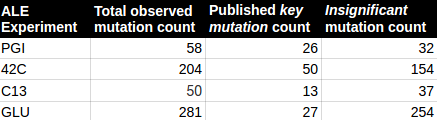
\includegraphics[width=0.8\textwidth]{class_imbalance_table.png}
  \label{tab:class_imbalance_table}
\end{table}
In establishing our classification evaluation metrics, we observe that there are many more insignificant mutations than key mutations, or in other words, there exists a class imbalance. We demonstrate this imbalance in Table \ref{tab:class_imbalance_table}. All but the PGI ALE experiment have an obvious class imbalance. Relying on accuracy alone to measure classification performance with a class imbalance can be misleading since one could naively classify all mutations as the majority class of the imbalance and still obtain a high accuracy. We consider avoiding the exclusion of significant mutations from our results as our highest priority; in other words, we consider \textit{recall} as our primary performance metric. In performing with high recall, we can better ensure that all key mutations are returned in our results, therefore providing the best identification of all significant genomic regions in an experimental evolution. Avoiding insignificant mutations in our results is of secondary importance since they can be later excluded by secondary manual investigations performed by the experimentalist. We will use \textit{precision} as the metric to evaluate our approach's ability to avoid insignificant mutations in our results.
\subsubsection{PGI ALE Experiment}
% * <pphaneuf@eng.ucsd.edu> 2016-08-13T20:14:33.404Z:
%
% "The gene PGI catalyzes the isomerization of glucose 6-phosphate to fructose 6-phosphate in upper glycolysis. Removal of this gene forces the glycolytic flux through the pentose phosphate pathway, creating a redox imbalance due to excess NADPH production ."
%
% ^.
The PGI ALE experiment and publication focused on the observed adaptive mutations selected for during an experimental evolution due to knocking out the phosphoglucose isomerase PGI gene from the K-12 MG1655 strain of \textit{E. coli}. The PGI gene plays a major role in the central metabolism of \textit{E. coli} and is a good candidate for studying how a strain learns to compensate for a loss of such significant impact. The experiment executed 10 parallel ALEs on replicates of \textit{E. coli} K-12 MG1655 lacking the PGI gene using ALE methodologies for 50 days in minimal media. Clones were taken from each ALE's final flasks and their mutations were defined by first whole-genome sequencing through both Nimblegen hybridization-base tiling arrays and Illumina Solexa technologies, then leveraging the Nimblegen's built-in variant calling capabilities and in-house software. PCR and Sanger sequencing was additionally used to verify mutations identified and the entire sequence of host genomic regions \cite{10.1371/journal.pgen.1001186}. Our analysis of the PGI ALE experiment samples was executed by processing the same reads generated by the authors using the Breseq 0.23 software pipeline against the \textit{E. coli} K-12 MG1655 reference genome (NCBI accession NC\_000913.2).
% * <pphaneuf@eng.ucsd.edu> 2016-09-22T00:24:29.708Z:
%
% Why was PGI 9 not included in the paper?
%
% ^ <pphaneuf@eng.ucsd.edu> 2016-09-22T03:16:46.041Z:
%
% Adam has responded with the idea that they believed something was poor about their resequencing and therefore they didn't included it in the analysis. Not a problem for this thesis since no significant mutation analysis used PGI 9 data.
%
% ^ <pphaneuf@eng.ucsd.edu> 2016-09-22T16:53:17.283Z.
\begin{table}[H]
  \centering
  \caption{PGI ALE experiment key mutation genomic region matching summary between the paper and the ALE Analytics automated enrichment key mutation analysis.}
  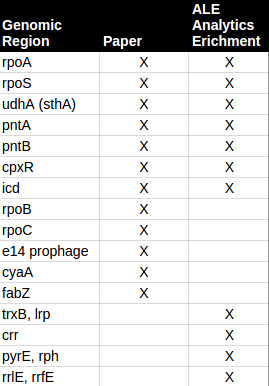
\includegraphics[width=0.45\textwidth]{pgi_key_mutation_regions.png}
\end{table}
The PGI ALE experiment paper doesn't explicitly list the key mutations as does the other ALE experiment papers involved in our evaluation. We therefore rationalize the paper's key mutations according to the findings presented on each mutation and their host genomic region. The PGI experiment publication identified the perturbation of the following genes as being important for the experiment's observed fitness:
\begin{itemize}
\item \textit{rpoS}: mutations observed suppresses stress response by modulating transcription; likely fitness selection in relation to the adaptation to loss of PGI.
\item \textit{rpoA}, \textit{rpoB}, \textit{rpoC}, \textit{cpxR} and \textit{cyaA}: mutations observed result in global network-level transcriptional regulation adaptations.
\item \textit{sthA}, \textit{pntA}, \textit{pntB}: mutations observed counter the redox imbalance of excess NADPH production due to PGI knockout.
\item \textit{e14 prophage deletion}: target and mutations observed are mechanistically unknown, yet experimental data shown to provide fitness.
\end{itemize}
The authors speculate that the deletion of the \textit{e14 prophage} is a unique contributor to the fitness of its host strain. This was determined due to not being able to reproduce the fitness of the host strain with any combination of other key mutations in followup ALEs. The \textit{e14 prophage} deletion manifests as unassigned missing coverage in our mutation reports, which we include in our ALE Analytics database but currently do not yet include in reports. The authors do mention the potential importance of the \textit{icd} SNPs coinciding with this deletion. It is speculated that these SNPs may have a fitness benefit in their potential to induce better translation efficiency to \textit{icd}. Due to the high frequency of these \textit{icd} SNPs, the enrichment analysis did include them in its results as key mutations. Though no solid evidence could be found on the \textit{icd} allele's fitness benefit, since the authors speculate that the \textit{icd} mutations are significant and the objective of the ALE Analytics automated analysis is to highlight the mutation that may be a result of the ALE's selective pressures, we consider the paper's \textit{icd} SNPs to be key mutations.

Of the 12 key mutations alleles published in the paper, the enrichment analysis is successful in finding 7. The ALE Analytics enrichment analysis finds multiple \textit{icd} alleles in both ALE 1 and ALE 5. \textit{icd} alleles were reported to be associated with the \textit{e14 prophage } deletion, published as occurring in the ALE 1. The evidence of high \textit{icd} enrichment in ALE 5 motivated an investigation into the possibility of an ALE 5 \textit{e14 prophage} deletion that was in fact found by manually investigating the missing coverage artifacts of the Breseq reports. This investigation serves to demonstrate the importance of automating key mutation identification for ALE experiments.

A minority of the published key mutations which didn't manifest more than once were included in the paper's key mutation set according to their functional association with significantly enriched genes. SNPs uniquely affecting transcription modulation genes \textit{cyaA}, \textit{rpoB}, and \textit{rpoC} were included as key mutations in the paper in addition to the mutations of the more frequently mutated \textit{rpoA}, \textit{rpoS} and \textit{cpxR} genes. These key mutations could be included in future enrichment analysis implementations by additionally considering the mutational enrichment of functional groups rather than only single genes.

The \textit{fabZ} SNP was speculated as important by the authors due to their knowledge of the potential metabolic perturbations caused by the PGI knockout and the idea that the this mutation may reduce its impact. This type of key mutation could be included in future enrichment analysis by including functional data on any type of perturbation introduced into the initial strain of the experimental evolution and identify mutations affecting genes functionally related to the initial perturbation. This approach would therefore also leverage the enrichment of functional groups of genes.

Published mutations in the \textit{rep}, \textit{yfeH}, \textit{fruK}, \textit{rodA}, \textit{bipA} and \textit{ispU} genes only manifest once and weren't discussed by the publication as being key mutations. These mutations were therefore not considered for either the publication's significant mutation set and the ALE Analytics enrichment analysis evaluation.

The ALE Analytics enrichment mutation analysis found 3 additional possible significant genomic regions described in Table \ref{tab:pgi_new_enrichment_muts} due to their frequency of mutation. Though these new enriched genomic regions contributed to the lessening of the enrichment analysis' precision metric, they present an opportunity for identifying further significant adaptations not caught by the authors.
\begin{table}[H]
  \centering
  \caption[New PGI ALE experiment enrichment key mutations found by the automated enrichment analysis.]{ The value 1 used to denote the presence of a mutation describes the approximate frequency in which the mutation was found within the sample population represented in the sample reads \cite{breseq_paper}.}
  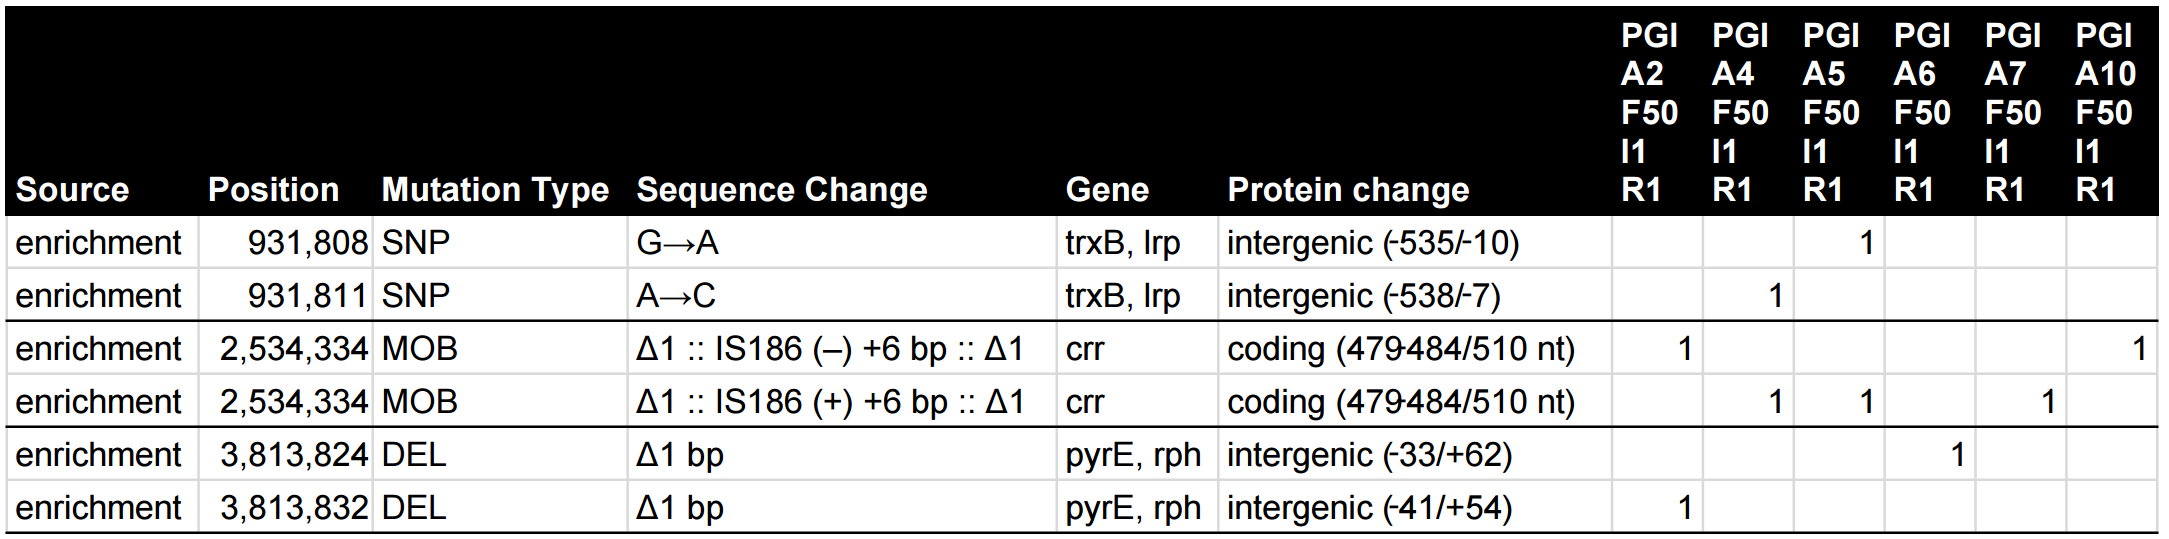
\includegraphics[width=\textwidth]{pgi_new_enrichment_muts.png}
  \label{tab:pgi_new_enrichment_muts}
\end{table}
No fixed mutations can be established with the PGI ALE experiment data set since all samples are endpoints of different ALEs and therefore do not provide any mutation time-course information for the fixed mutation analysis to work with.
\begin{table}[H]
  \centering
  \caption{PGI ALE experiment classification performance.}
  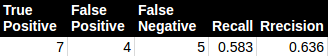
\includegraphics[width=0.6\textwidth]{pgi_precision_recall.png}
\end{table}
\subsubsection{42C ALE Experiment}
The 42C ALE experiment and publication focused on the observed adaptive mutations selected for during an experimental evolution with a selective pressure of a culture temperature of 42$^{\circ}$C. The experiment executed 10 parallel ALEs on replicates of \textit{E. coli} K-12 MG1655 for 45 days in minimal media. Clones were taken from each ALE's final flask, sequenced using the Illumina MiSeq platform and their mutations defined using whole genome re-sequencing with the Breseq 0.22 software pipeline against the \textit{E. coli} K-12 MG1655 reference genome (NCBI accession NC\_000913.2) \cite{pmid25015645}.

The authors of the 42C paper considered key mutations as those that perturbed a gene in more than one ALE endpoint. Their key mutation results were clearly annotated in a Table 2 \cite{pmid25015645}. This ALE experiment experienced two different hypermutator strains, proposed as independently manifesting in ALE 2, where \textit{mutL} was mutated, and ALE 6, where \textit{dnaQ} was mutated. The ALE 2 hypermutator strain went on to contaminate ALE 3 and the hypermutator strain in ALE 6 went on to contaminate ALE 8. Due to this contamination, the authors didn't consider mutations recurring between ALE endpoints derived from the same hypermutator strain as key mutations. The authors recognized unique mutations occurring within the same genomic region within and between hypermutator strain pairs and therefore did not completely disregard the hypermutator samples.
\begin{table}[H]
  \centering
  \caption{The 42C ALE experiment {key mutation} genomic region matching summary between the paper and the ALE Analytics automated key mutation analysis.}
  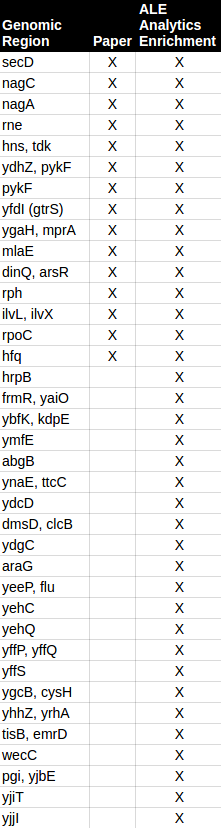
\includegraphics[width=0.3\textwidth]{42c_key_mutation_regions.png}
\end{table}
The ALE Analytics enrichment key mutation analysis finds all 14 of the genomic regions affected by the published key mutations. The ALE Analytics enrichment analysis is successful in finding all key mutations because its implementation is partly based on the key mutation protocol establish by this paper.
\begin{table}[H]
  \centering
  \caption[New enrichment key mutations found by the automated analysis]{New enrichment key mutations found by the automated analysis. ALE endpoint pair (2, 3) and (6, 8) are each derived from the same hypermutator strain, therefore explaining the large amount of mutations shared between the endpoints. The value of 1 used to denote the presence of a mutation describes the approximate frequency in which the mutation was found within the sample population represented in the sample reads \cite{breseq_paper}.}
  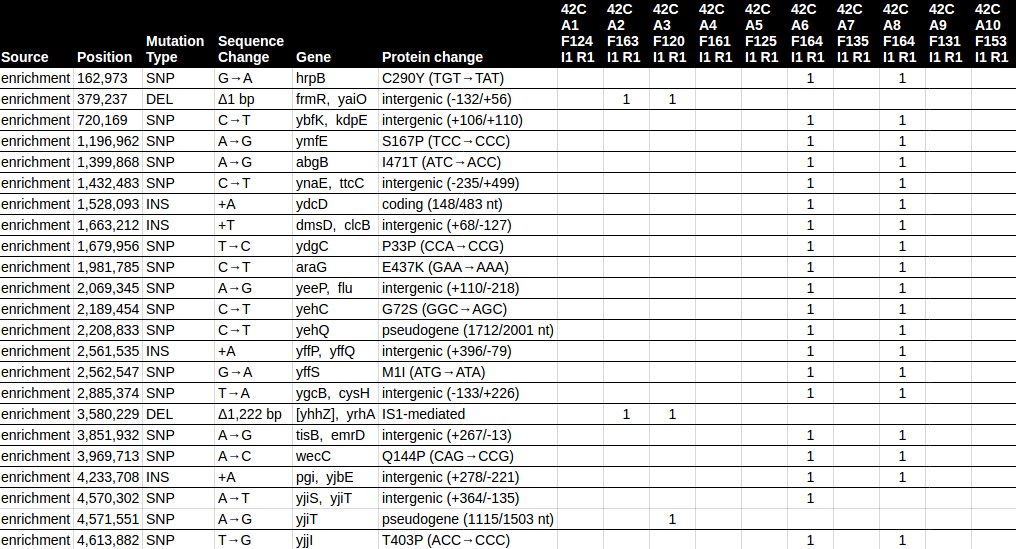
\includegraphics[width=\textwidth]{42c_new_enrich_muts.png}
\end{table}
The ALE Analytics enrichment mutation analysis finds 22 additional genomic regions affected by more than one mutation. The \textit{mutL} and \textit{dnaA} mutations mentioned by the paper as the cause for ALE 2, 3, 6 and 8 endpoints to become hypermutators were included in the automated analysis' enrichment key mutations. The paper does not include these in their table of key mutations, though do describe their importance; we therefore do not consider the \textit{mutL} and \textit{dnaA} mutations as false positives.

These 22 additional genomic regions of interest only manifest in the ALEs that have been identified by the authors as being overcome by the same hypermutator strain except for the \textit{yjiT} alleles. \textit{yjiT} was mutated in the ALE 3 and 6 endpoints, hypermutators of separate origins, and therefore make its mutations candidate for classification as key mutations. The exclusion of the \textit{yjiT} mutations in the author's key mutation set may have been an oversight in their manual workflow; the automated enrichment key mutation analysis will reduce the possibility for these errors with its future usage. If our evaluation were to exclude hypermutator mutations from both the published significant mutation set and our results, both the subsets of the published non-hypermutator and automated analysis key mutations would match without any additional key mutations. 

The obvious contamination made clear by the amount of hypermutator mutations in contaminated strains lends us intuition on how to automate the identification of contamination among samples. Additionally, one could automate the identification of contamination among samples by  recognizing when samples share a large subset of the exact same point mutations.

No fixed mutations can be established with the 42C ALE experiment data set since all samples are endpoints of different ALEs and therefore do not provide any mutation time-course information for the fixed mutation analysis to process.
\begin{table}[H]
  \centering
  \caption{The 42C ALE experiment classification performance.}
  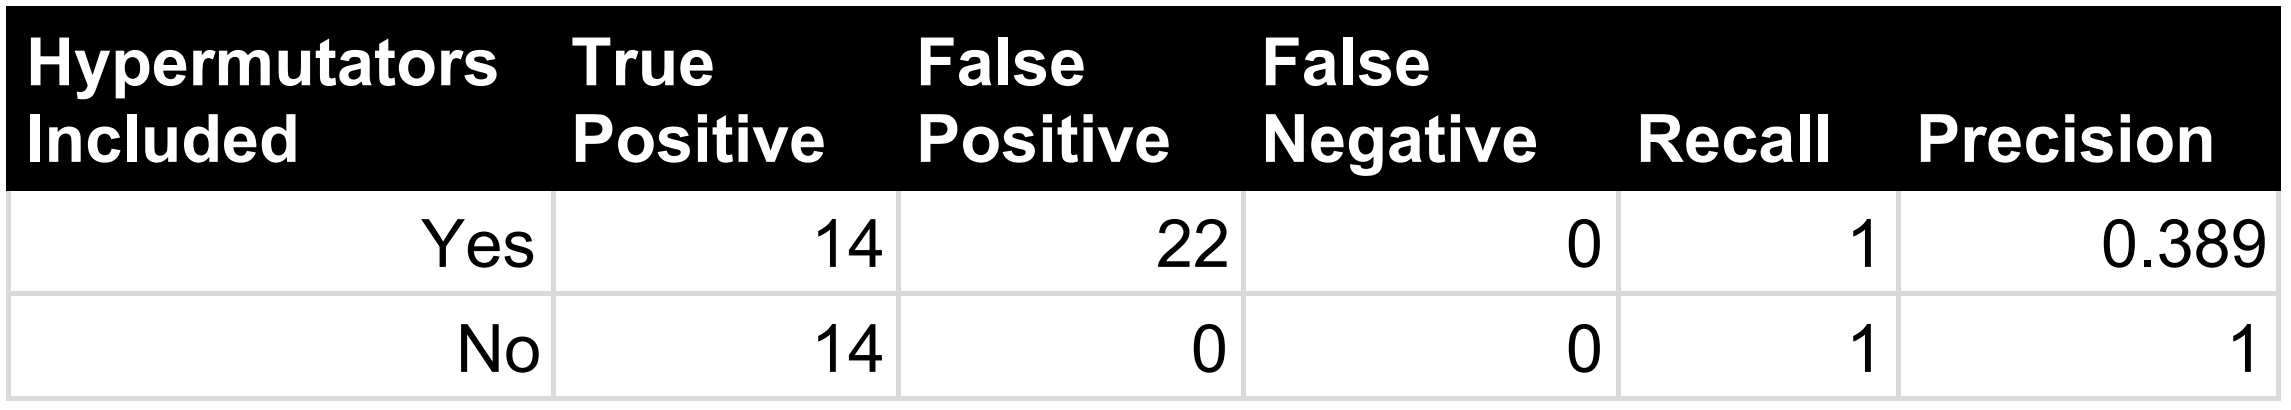
\includegraphics[width=0.8\textwidth]{42c_precision_recall.png}
\end{table}
\subsubsection{C13 ALE Experiment}
The C13 ALE experiment and publication focused on the observed adaptive mutations selected for during an experimental evolution using \textsuperscript{13}C-glucose as a carbon source for \textit{E. coli} growth. The key mutations found by this experiment were compared to those of \cite{pmid25304508}, which uses \textsuperscript{12}C-glucose, to investigate if there is any evidence of differing adaptations and therefore additional metabolic stress from using the \textsuperscript{13}C-glucose isotope. The experiment executed 6 parallel ALEs  on replicates of \textit{E. coli} K-12 MG1655 for approximately 1000 generations per ALE. Two clonal samples were taken from each ALE; one sample served as a midpoint clone and the other as the endpoint clone. The clones were sequenced using the Illumina MiSeq platform and their mutations defined using whole genome re-sequencing with the Breseq 0.23 software pipeline against the \textit{E. coli} K-12 MG1655 reference genome (NCBI accession NC\_000913.2).

The authors of the C13 published material considered the mutations for genes that were enriched in more than one endpoint to be key mutations. Their key mutation results were clearly stated as those mutations which affected the \textit{pyrE/rph}, \textit{rpoB}, \textit{hns/tdk} and \textit{rhsE} genomic regions. The ALE Analytics enrichment key mutation analysis finds all 4 of the published genomic regions affected by key mutations.
\begin{table}[H]
  \centering
  \caption[New C13 ALE experiment enrichment key mutations.]{ The value of 1 used to denote the presence of a mutation describes the approximate frequency in which the mutation was found within the sample population represented in the sample reads \cite{breseq_paper}}
  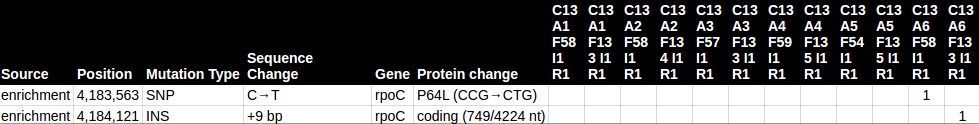
\includegraphics[width=0.9\textwidth]{c13_new_enrich_muts.png}
  \label{tab:c13_new_enrich_muts}
\end{table}
The ALE Analytics enrichment mutation analysis found 1 additional possible significantly enriched allele described in Table \ref{tab:c13_new_enrich_muts}: \textit{rpoC}. The authors did not include \textit{rpoC} mutations as a key mutation since their approach was limited to high frequency alleles among different ALEs. The ALE Analytics enrichment analysis additionally returns mutations found to affect genomic regions within multiple samples of the same ALE.

The ALE Analytics fixed mutation analysis finds 2 of the 4 published key mutation alleles; those key mutations missed were due to only manifesting in ALE endpoint samples. The ALE Analytics ascending frequency fixed mutation analysis finds the same results. If the C13 ALE experiment had more midpoint samples, the fixing of these mutations may be more evident and would ultimately be captured by the fixed key mutation analysis. Significant mutations should ultimately be all caught by the fixed key mutation analysis with enough samples, though the question that remains is how many samples from an ALE are adequate to provide enough resolution on mutation lineages to capture all fixing mutations.
\begin{table}[H]
  \centering
  \caption{The C13 ALE experiment {key mutation} genomic region matching summary between the paper and the ALE Analytics automated key mutation analyses.}
  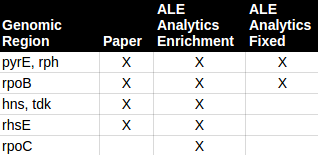
\includegraphics[width=0.6\textwidth]{c13_key_mutation_regions.png}
\end{table}
\begin{table}[H]
  \centering
  \caption{The C13 ALE experiment classification performance.}
  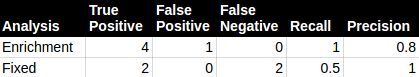
\includegraphics[width=0.7\textwidth]{c13_precision_recall.png}
\end{table}
\subsubsection{GLU ALE Experiment}
% * <pphaneuf@eng.ucsd.edu> 2016-10-23T04:30:15.025Z:
%
% NOTE: Adam had mentioned that ALE 5 was contaminated, though it was still used in the paper for identifying key mutations. Will therefore keep it in my analysis also.
%
% ^.
The GLU ALE experiment and publication focused on establishing and leveraging novel ALE methods and observing the adaptive mutations selected for using these ALE methods and \textit{E. coli} on glucose minimal media at 37$^{\circ}$C. This experiment isolated the selection pressure to the growth rate of the strain by propagating batch cultures to new flasks during their exponential growth phase rather than the stationary growth phase; this avoids the fixing of mutations that grant fitness to attributes other than growth rates. The experiment executed 8 parallel ALEs on replicates of \textit{E. coli} K-12 MG1655, capturing samples from both the final and intermediate ALE flasks for whole genome sequencing with the Illumina MiSeq platform and re-sequencing using the Breseq 0.23 software pipeline against the \textit{E. coli} K-12 MG1655 reference genome (NCBI accession NC\_000913.2).

The authors employed two strategies for identifying key mutations. The first was to find genomic regions that were mutated in the endpoint of multiple ALEs.
The second was to identify genomic regions within an ALE that experienced the replacement of one mutation with another; both mutations involved were considered key mutations.
\begin{table}[H]
  \centering
  \caption[A combination of the new enrichment and fixed key mutations found by the automated analysis.]{ The only difference between the two sets is that the fixed key mutation set does not include the \textit{wecA} alleles.}
  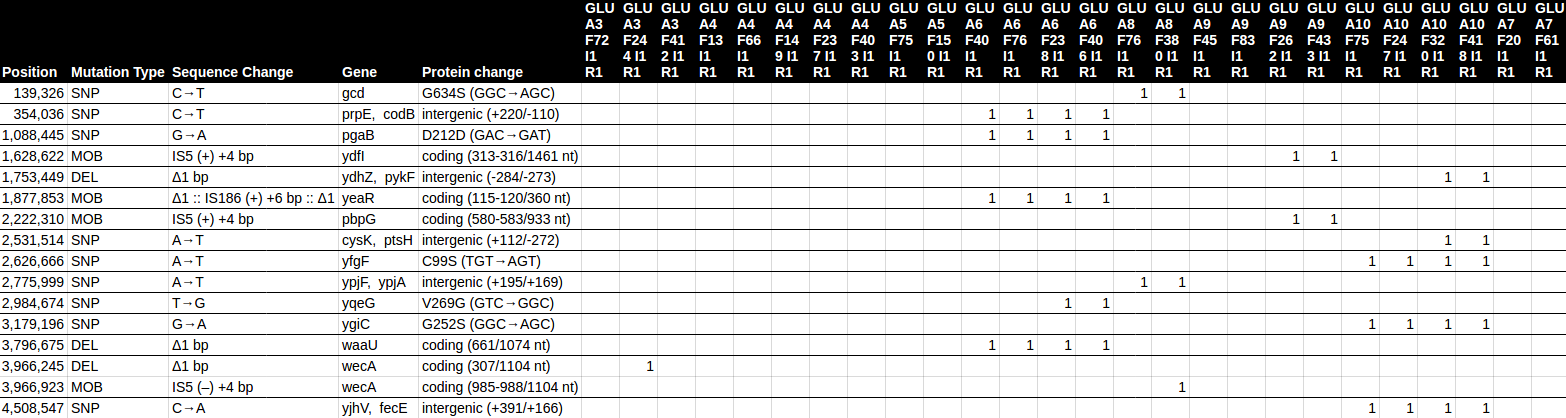
\includegraphics[width=\textwidth]{glu_new_enrich_fix_muts.png}
  \label{tab:glu_new_enrich_fix_muts}
\end{table}
The ALE Analytics enrichment key mutation analysis finds all 8 of the genomic regions affected by the published key mutations. This analysis also finds 15 additional possible significant genomic regions, described in Table \ref{tab:glu_new_enrich_fix_muts}, due to the frequency in which many mutations reoccurred within an ALE. The ALE Analytics fixed key mutation analysis finds 14 unpublished key mutations. The ascending frequency fixed mutation analysis finds the same results. The subset of unpublished fixed mutations are identical to the subset of unpublished enrichment mutations, with the exception of \textit{wecA}. The \textit{wecA} alleles do manifest in such a way that conforms to the key mutation protocol published for this ALE experiment, though were not included in the paper's key mutation results. Besides the \textit{wecA} alleles, the new key mutations were not published by the authors as being significant since they did not exhibit the criteria of mutating the same genomic region in more than one ALE or replacing a mutation within an ALE. Though the new key mutation genomic regions contributed to the lessening of the enrichment and fixed key mutation analysis' precision metric, they present an opportunity for identifying further significant adaptations not identified by the authors.
\begin{table}[H]
  \centering
  \caption{The GLU ALE experiment {key mutation} genomic region matching summary between the paper and the ALE Analytics automated key mutation analysis.}
  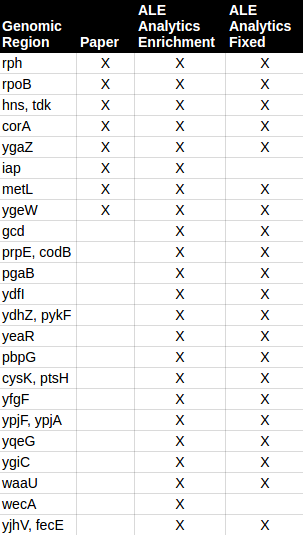
\includegraphics[width=0.5\textwidth]{glu_key_mutation_regions.png}
\end{table}
\begin{table}[H]
  \centering
  \caption{The GLU ALE experiment classification performance.}
  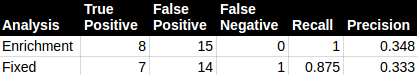
\includegraphics[width=0.7\textwidth]{glu_precision_recall.png}
\end{table}

\clearpage
I would like to acknowledge Dr. Adam Feist, Dr. Ryan LaCroix, Troy Sandberg, Gabriela Guzman, Joon Ho Park, Colton Llyod, Douglas McCloskey and the many others who have contributed their experiment data to enable the work of this thesis.

\chapter{Discussion}
% * <pphaneuf@eng.ucsd.edu> 2016-08-13T23:22:12.398Z:
%
% "A persistent challenge and goal in ALE experiments is differentiating between causal mutations and genetic hitch-hikers. 57% (30 of 53) of all mutations persisted in every subsequent clone examined until the experiment ended (mutations only observed in the last clone examined for each experiment were not considered)." -GLU 
%
% ^ <pphaneuf@eng.ucsd.edu> 2016-08-13T23:22:45.381Z:
%
% This is why we need more than 1 method of identifying key mutations.
%
% ^.
% * <pphaneuf@eng.ucsd.edu> 2016-10-11T02:20:54.338Z:
%
% The fixating mutations analysis possibly returns a more refined list of key mutations due to its design of focusing on a particular mutational pattern, though this analysis can't differentiate between fixating mutations selected for their fitness benefits and hitchhiking mutations.
%
% ^.
% * <pphaneuf@eng.ucsd.edu> 2016-10-18T21:50:21.977Z:
%
% Target: ALE Mutation Database, Inputs: ALE experiment mutations, ALE experiment metadata, ALE experiment duplications.
%
% ^.
\section{Key Mutation Analysis}
% * <pphaneuf@eng.ucsd.edu> 2016-08-15T03:48:44.482Z:
%
% Talk about why population samples conferred an advantage over only using clonal samples.
%
% ^ <pphaneuf@eng.ucsd.edu> 2016-08-16T17:38:45.092Z:
%
% This is detailed in the GLU paper.
%
% ^.
The implementation of our automated analysis aims to distill the multiple methods published in identifying key mutations, though each of these published methods make no guarantee of including all significant mutations or excluding artifacts such as hitchhiker mutations \cite{pmid25304508}. A successful key mutation analysis will ultimately leverage multiple factors to judge a mutation's significance in an ALE experiment. Additional factors to those we have implemented in this thesis would be ALE growth rate profiles and gene functional group mutational enrichment.

In executing an evolution, the ALE Machine must track the growth rate of sample for its operations. The compilation of these growth rates contain vital fitness data for the experiment, such as which sample manifested a jump in growth rate during an ALE. Mutations in a population that occur immediately before the growth rate jump and gain dominance once the growth rate stabilizes are likely candidates for key mutations. This fitness data can be integrated into key mutation analysis to serve as an additional dimension in judging the significance of a mutation \cite{pmid25304508}. Mutations can also be evaluated according to if their host gene is functionally similar to other mutated genes or is associated with the selection pressure such as experimental conditions or initial perturbations. This list of factors ultimately describe the many additional dimensions that can be further incorporated into automatically evaluating whether a mutation is strongly correlated to the selection pressures of an evolution.

The enrichment key mutation analysis rendered the best classification performance for this thesis; this was likely due to the small amount of samples per ALE with the ALE experiments used in the evaluation. Future ALE experiments may be enabled by ALE Analytics to incorporate more samples per ALE, with each sample being a population rather than clone. In general, more samples would grant more data points in the time-course of an evolution, allowing for more mutation data to describe the evolution. If these samples were populations, our analysis would be able to investigate the population dynamics of evolutions and track not only the consensus mutations but the balance of mutations found in only subsets of the entire population. This higher resolution of samples would enable the fixed key mutation analysis to have a higher probability of finding fixed mutation patterns. The enrichment key mutation analysis may ultimately be identifying mutations that, with more samples, would be identified with fixed key mutation analysis. The fixed key mutation analysis is more clear and intuitive in its intent in describing as to why a mutation may be significant, which is an advantage that the enrichment mutational pattern analysis lacks.

The work of this thesis justifies more population samples per evolution. Before this work, the decision on the sample count to sequence per ALE was based on investigating the genotypes of endpoint samples. Now that we have tools to quickly process a previously infeasible volume of samples, we have the opportunity to investigate new strategies in identifying key mutations and exploring population dynamics within experimental evolutions.
\section{Shared Enrichment and Fixed Mutations}
% We investigate if ALE Analytics features are able to find novel perspectives on the key mutations by leveraging the the fact that all ALE experiments are unified within one database and investigate if ALE experiments share any key mutations. 
A significant opportunity of the consolidation of ALE experiment reporting is that one can easily compare the mutations of multiple ALE experiments and search for mutational trends among all provided ALE experiments. We have leveraged this opportunity and implemented the \textit{shared enrichment} and \textit{shared fixed key mutation} features. These features leverage the nature of the ALE Analytics platform to automate the identification of genomic regions that share key mutations across ALE experiments. In this section, we present the shared enrichment and fixed mutations and elaborate on their significance.% We additionally incorporated population samples from the GLU ALE experiment; these samples were not previously considered in any of our analysis due to their exclusion from the published material's key mutation analysis.
\begin{table}[H]
  \centering
  \caption{Shared enrichment and fixed mutation genomic regions among all ALE experiments evaluated.}
  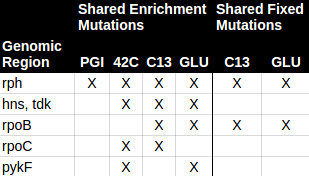
\includegraphics[width=0.55\textwidth]{shared_enrichment_fixed_genomic_regions.png}
\end{table}
\textit{rph} was host to enrichment and fixed key mutations in all ALE experiments used in our evaluation. The meta data for the samples hosting these key mutations shows us that each experiment shares a parent strain yet differ by a single feature. Besides the GLU project, these differing features describe the selection pressure on the experiments, therefore each ALE experiment sharing the \textit{rph} enrichment theoretically involves a different selection pressure. We can therefore conclude from the comparison of experimental conditions through the experiment meta data that the enrichment of \textit{rph} is a general optimization that the parent strain of these experiments can obtain when under any pressure. The \textit{rph} mutations seen in these ALE experiments are in fact thought to help manage a specific defect in the \textit{E. coli} K-12 MG1655 strain in which the starting strain for these ALE experiments derive from \cite{Conrad2009}.

The \textit{hns-tdk} intergenic region was the second most mutated among all enrichment mutations. This region along, with \textit{rpoB} and \textit{rpoC}, has been associated with global transcriptional regulation. Mutating these genes in some manner may have benefited a host's growth rate according to changes in transcription levels \cite{Kobayashi01011990, AYERS1989749, Cheng2014, Wang1445}. The GLU and C13 ALE experiments sharing the \textit{rpoB} enrichment and fixed mutations were in fact very similar in that the experiments were designed to select for growth rate, where C13 only differed in the isotope of the carbon source provided. These shared mutated key genomic regions therefore confirm the conclusion of the \cite{pmid26964043}, that the C13 carbon source does not significantly affect the host metabolism and therefore enabled the evolutions of the C13 and GLU ALE experiments to follow a significantly similar track.

The \textit{pykF} genomic region is enriched in the 42C and GLU ALE experiments. These experiments have very similar conditions beyond their sample temperatures. Mutations in \textit{pykF} have in fact been associated with enabling an increase in uptake of glucose by reducing or disabling the metabolism of phosphoenolpyruvate to pyruvate \cite{Woods13062006, 10.1371/journal.pgen.1001164, Blank25022014}. This fitness benefit is likely enabled by the fact that both experiments use M9 glucose minimal media, therefore providing an abundance of glucose to the populations.

\section{ALE Analytics Platform Feature Overview}
The ALE Analytics platform was built to support the analysis needs of its users; many features were therefore implemented to service various perspectives of analysis. This section presents an overview of the current capabilities of the ALE Analytics platform to exemplify how all current analysis features fit together.

% * <pphaneuf@eng.ucsd.edu> 2016-11-05T17:31:11.658Z:
% 
% TODO: explain the using a modern industrial strength technology stack on a dedicated server using production configurations and additionally leveraging industry standard HTTPS for securely encrypted web browsing.
% 
% ^.

On login, users are greeted with the ALE Analytics homepage, known as the \textit{dashboard}, which presents an overview of the mutational database currently available to the platform. This page presents the most frequently mutated genes, the most frequent mutation descriptions and the frequency of mutation types within the mutation database. An example of the dashboard can be seen in Figure \ref{fig:thesis_dashboard_page}. From the dashboard, users have access to their ALE experiments and all other platform features. Each ALE experiment has a similar home page with the same type of statistics as the dashboard. This page additionally includes alignment statistics for all experiment samples and a mutation needle plot \cite{michael_p_schroeder_2015_14561} for presenting the spread of mutations across the experiment's reference genome. Users can quickly gain a sense of mutation hot-spots in their experiment according to the mutation needle plot. The experiment home page is exemplified in Figure \ref{fig:experiment_stats_page}. From the ALE experiment home page, users have access to experiment specific applications, such as the experiment's mutation lineage and key mutation analysis reports. Users can also view a report of the meta data associated with each sample of an experiment, shown in Figure \ref{fig:metadata_page}. The experimental condition details, crucial to analysis, are contained within this meta data report.
\begin{figure}[H]
  \centering
  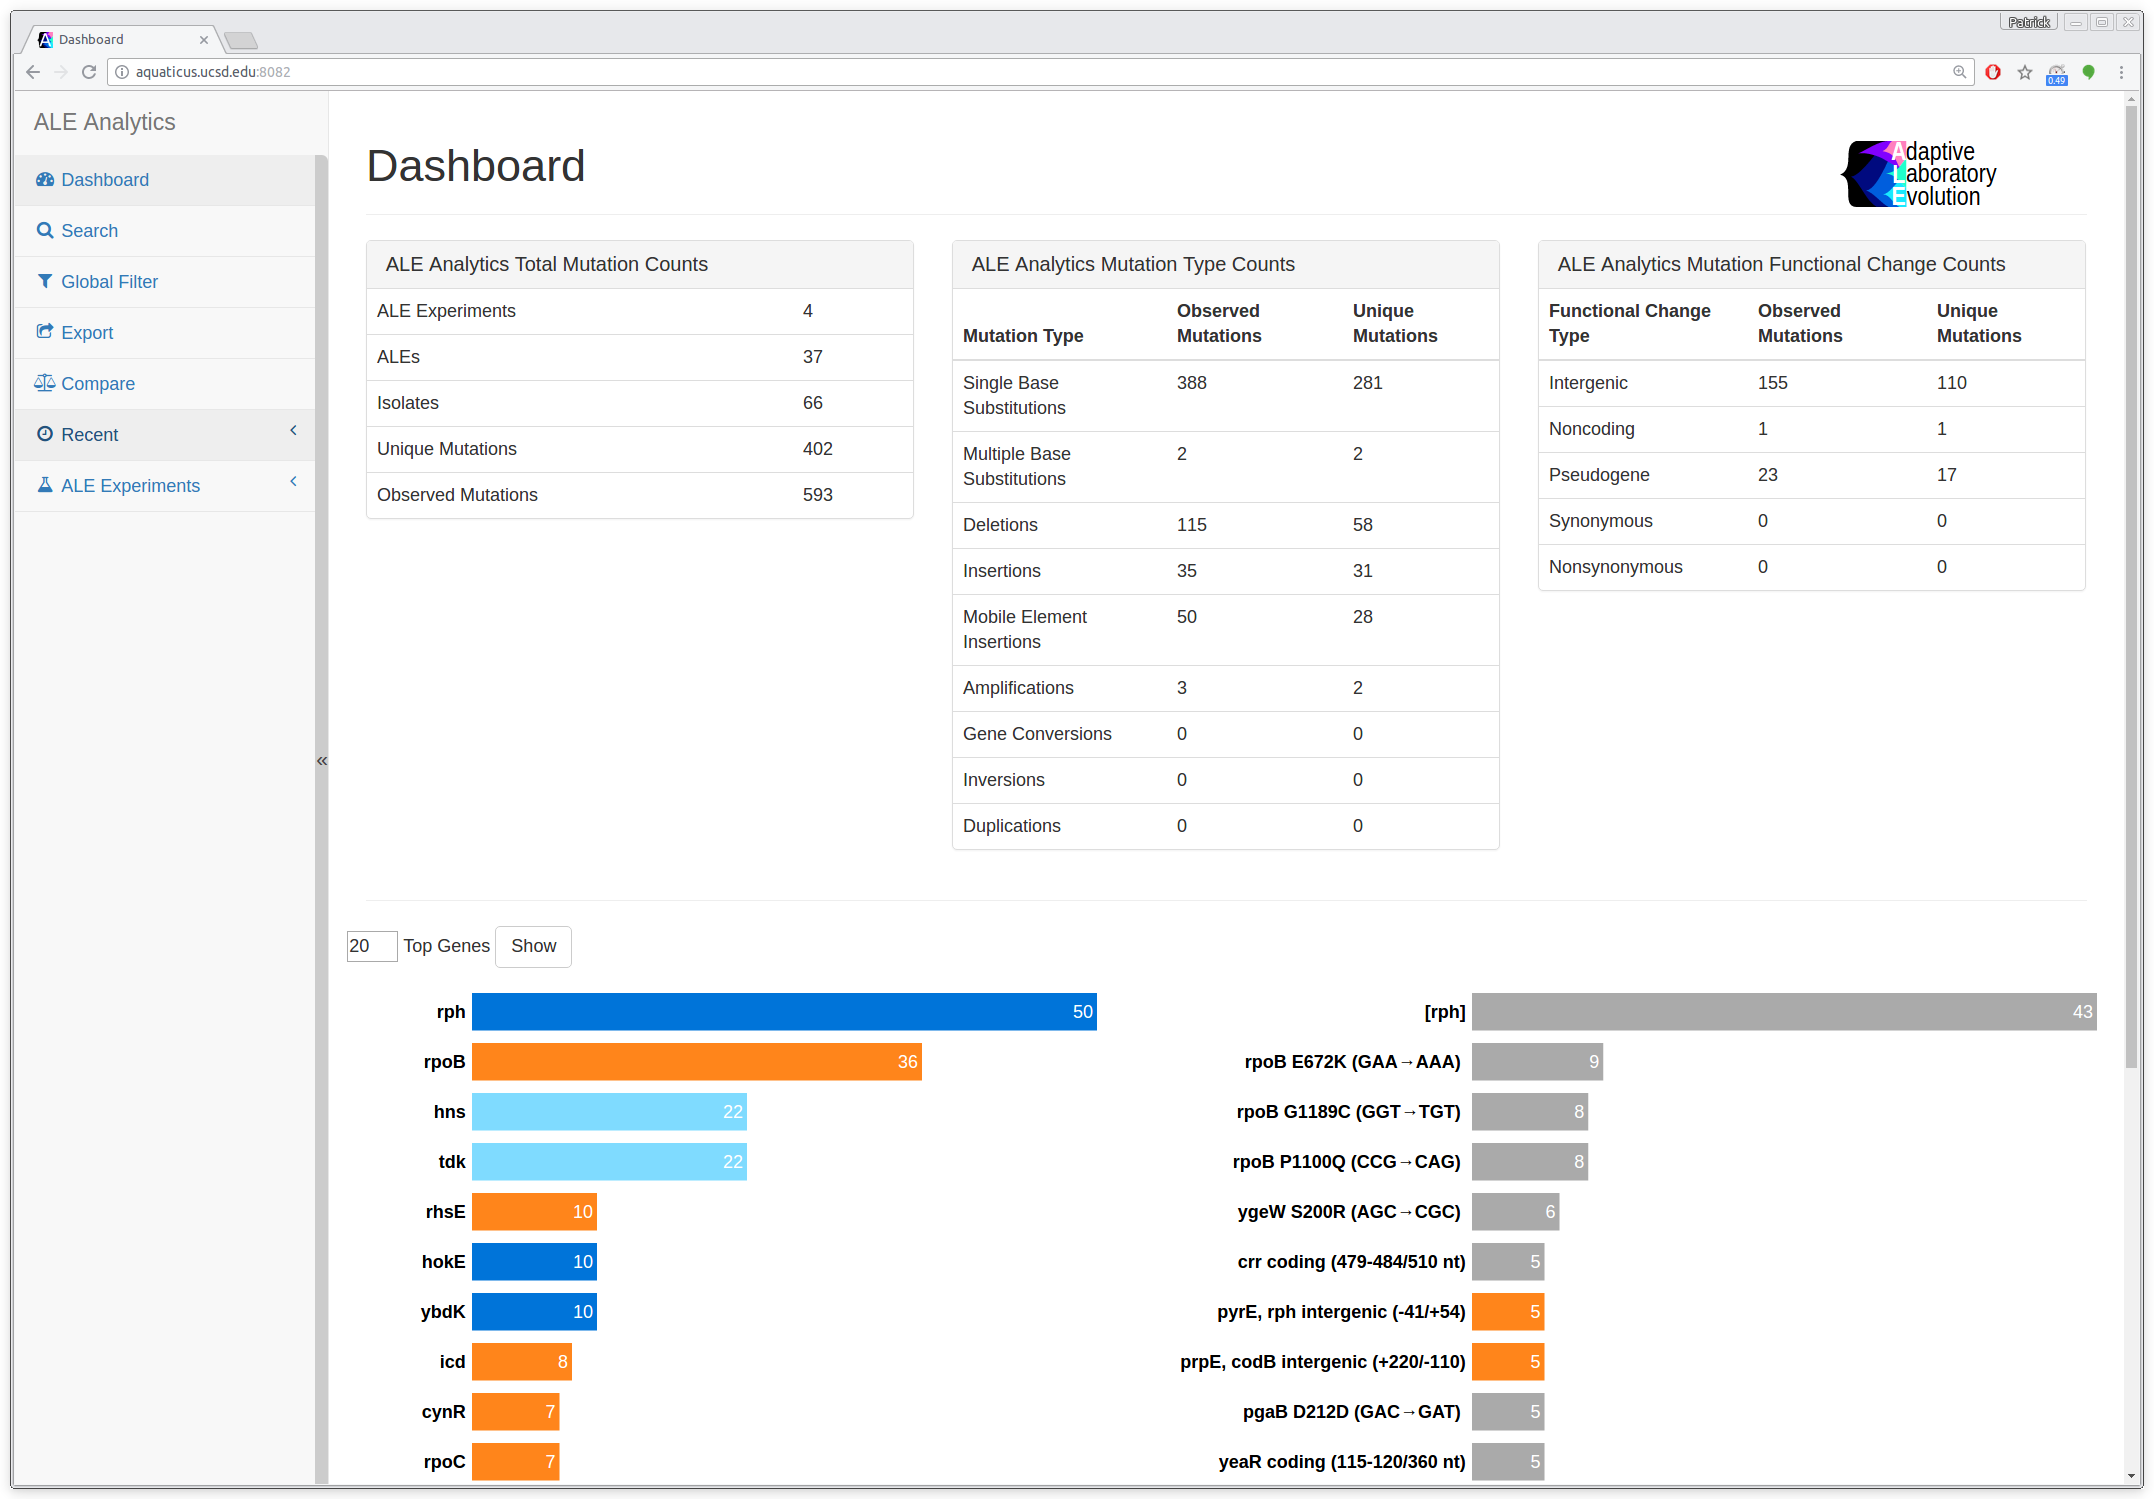
\includegraphics[width=0.9\textwidth]{thesis_dashboard_page.png}
  \caption{A screenshot of the dashboard for the instance of ALE Analytics used to accomplish the analysis contained within this thesis.}
  \label{fig:thesis_dashboard_page}
\end{figure}
\begin{figure}[H]
  \centering
  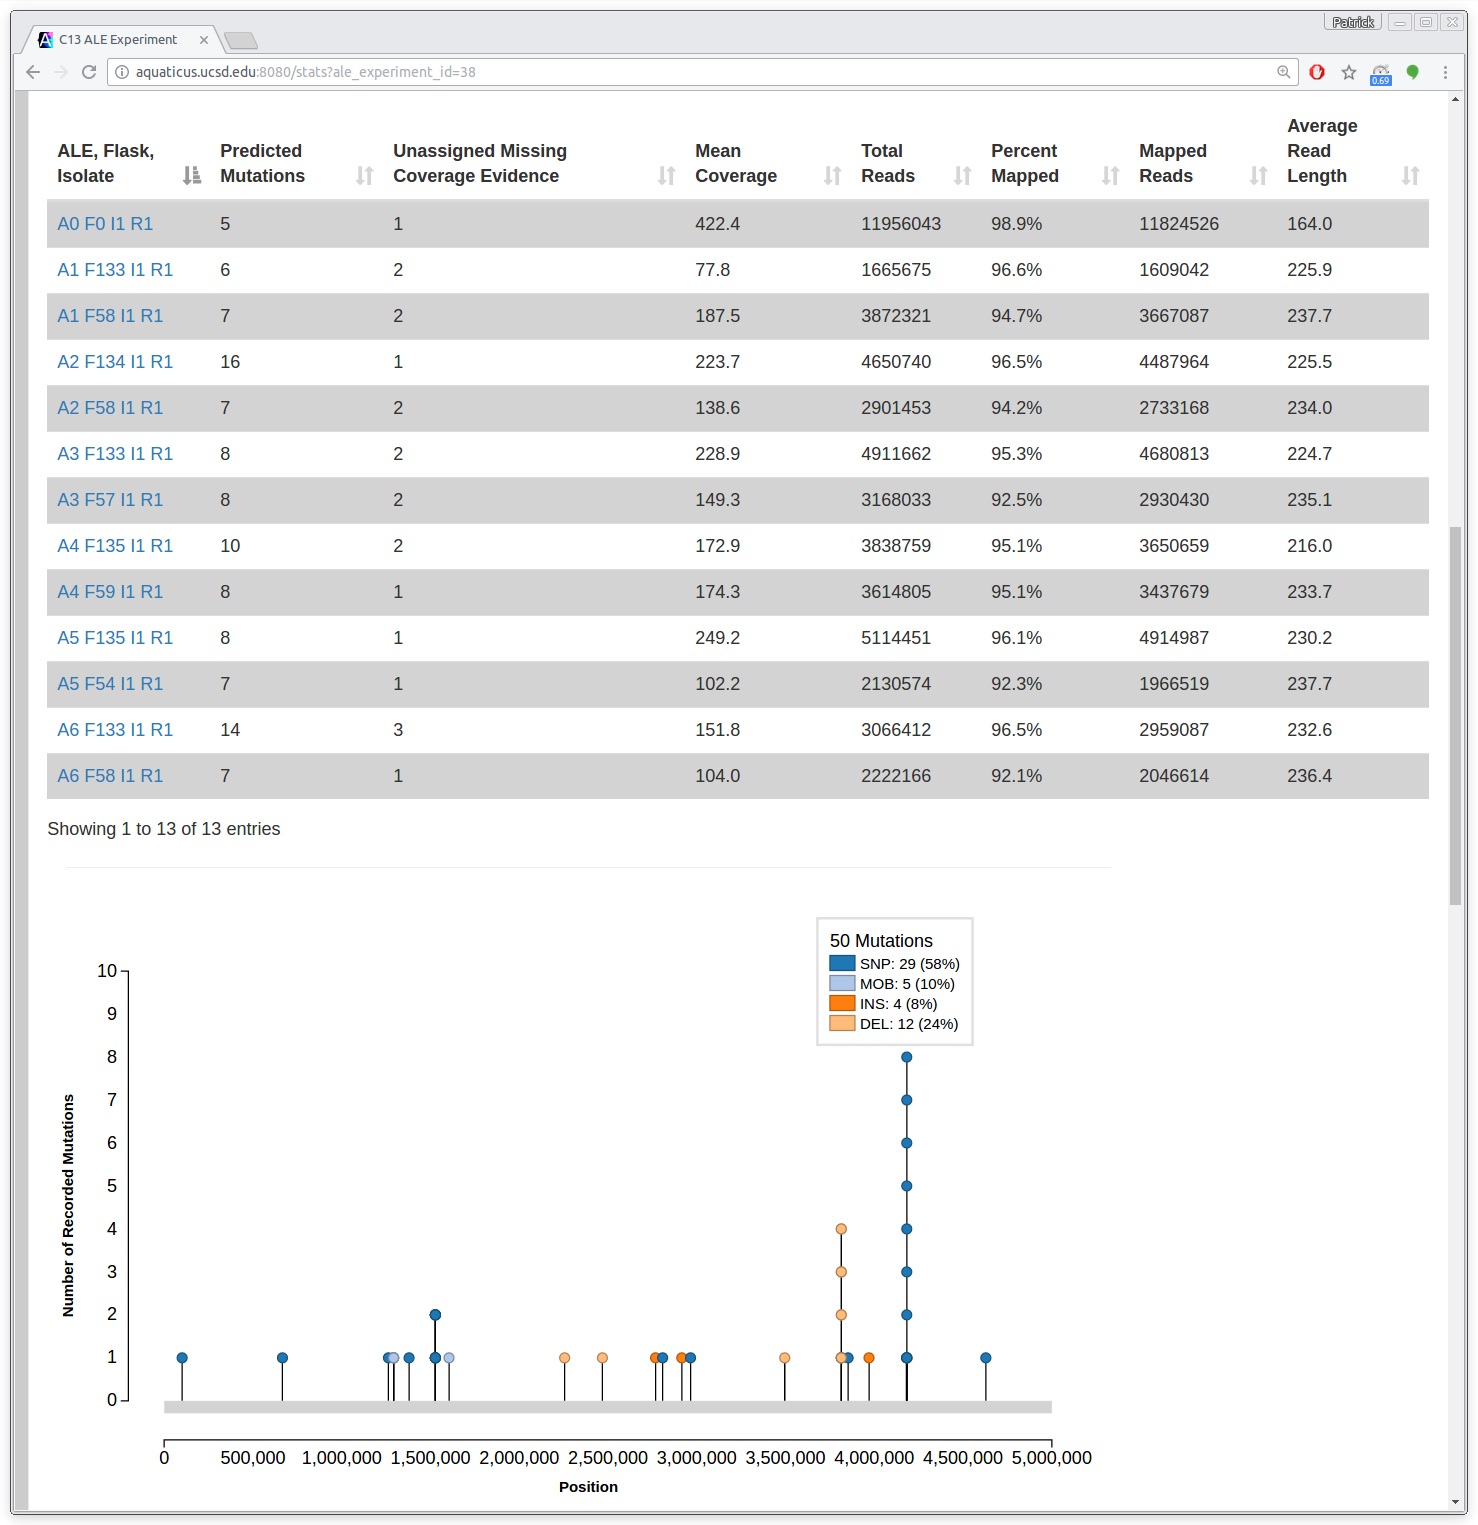
\includegraphics[width=0.9\textwidth]{experiment_stats_page.png}
  \caption{A screenshot of the C13 ALE experiment home page for the instance of ALE Analytics used to accomplish the analysis contained within this thesis.}
  \label{fig:experiment_stats_page}
\end{figure}
\begin{figure}[H]
  \centering
  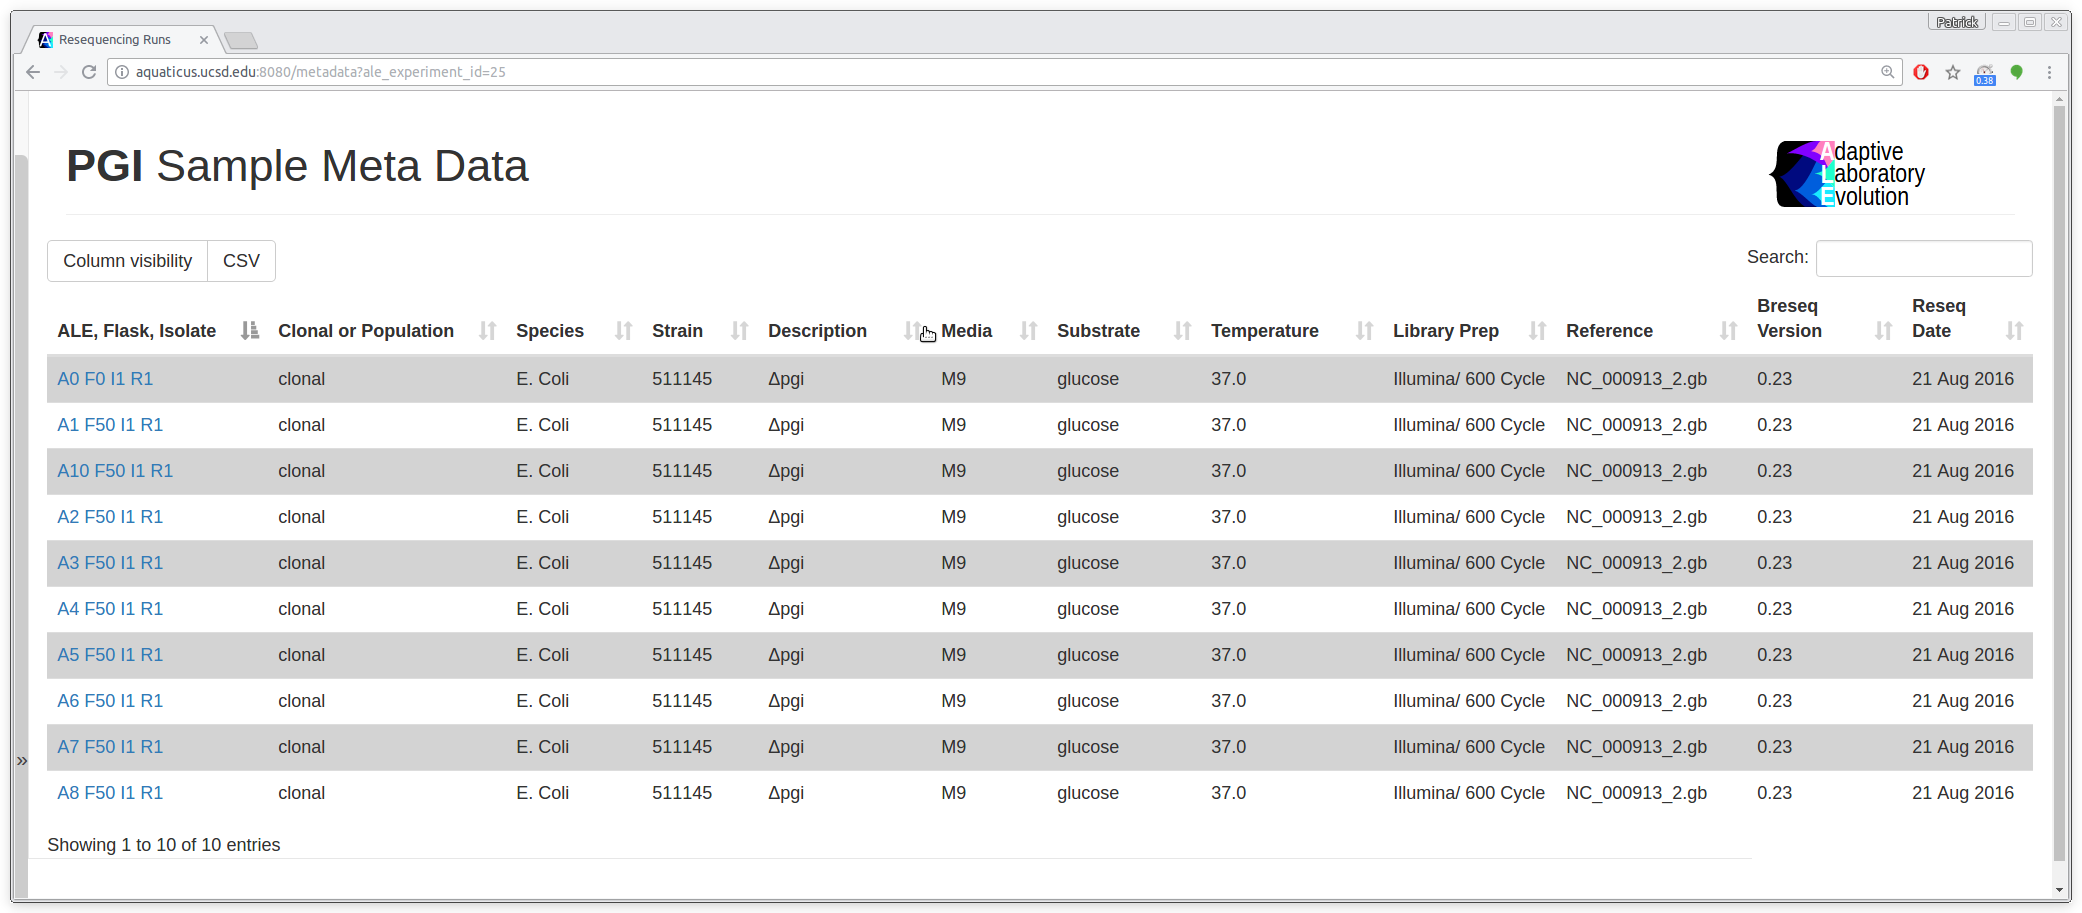
\includegraphics[width=0.9\textwidth]{metadata_page.png}
  \caption{A screenshot of the PGI ALE experiment's meta data for the instance of ALE Analytics used to accomplish the analysis contained within this thesis.}
  \label{fig:metadata_page}
\end{figure}
Users often need to compare ALE experiments to identify shared mutations. ALE Analytics includes a feature named \textit{compare} that will summarize the combination of ALE experiments similar to the experiments home page and build a mutation lineage reporting page from their combined mutations. Along with the mutation lineages, this feature builds the combined enrichment and fixed mutation tables, automating the comparison of the obvious significant mutations among compared ALE experiments.

Mutation filters play a critical role in all ALE experiment analysis. Both experimentalists and automated analysis require functionality that ignore mutations inappropriate for analysis. Mutations are often judged as inappropriate due to being identified as sequencing or alignment artifacts. Mutations can also be filtered on the basis of not containing any information pertaining to an experiment, such as those exhibited by an experiment's starting strain in relation to the reference genome used in alignment. We have defined two levels of filters: \textit{global} and \textit{experiment} levels. Global filters exclude the occurrence of a mutations for all ALE experiment analysis, where experiment filters ignore mutations for specific experiments. The parameters for global mutation filtering are unique mutations and genes. The parameters for experiment mutation filtering are unique mutations, genes, and observed mutation frequency. The experiment mutation filtering is shown in Figure \ref{fig:filter_page}.
\begin{figure}[H]
  \centering
  \includegraphics[width=0.9\textwidth]{filter_page.png}
  \caption{A screenshot of the PGI ALE experiment mutation filter page for the instance of ALE Analytics used to accomplish the analysis contained within this thesis.}
  \label{fig:filter_page}
\end{figure}
The compilation of all ALE experiments into one resource enables our ALE Analytics platform to implement a mutation search feature. This feature generates reports of mutations and their host samples according to a set of search parameters. An example of the search feature is shown in Figure \ref{fig:search_page}
\begin{figure}[H]
  \centering
  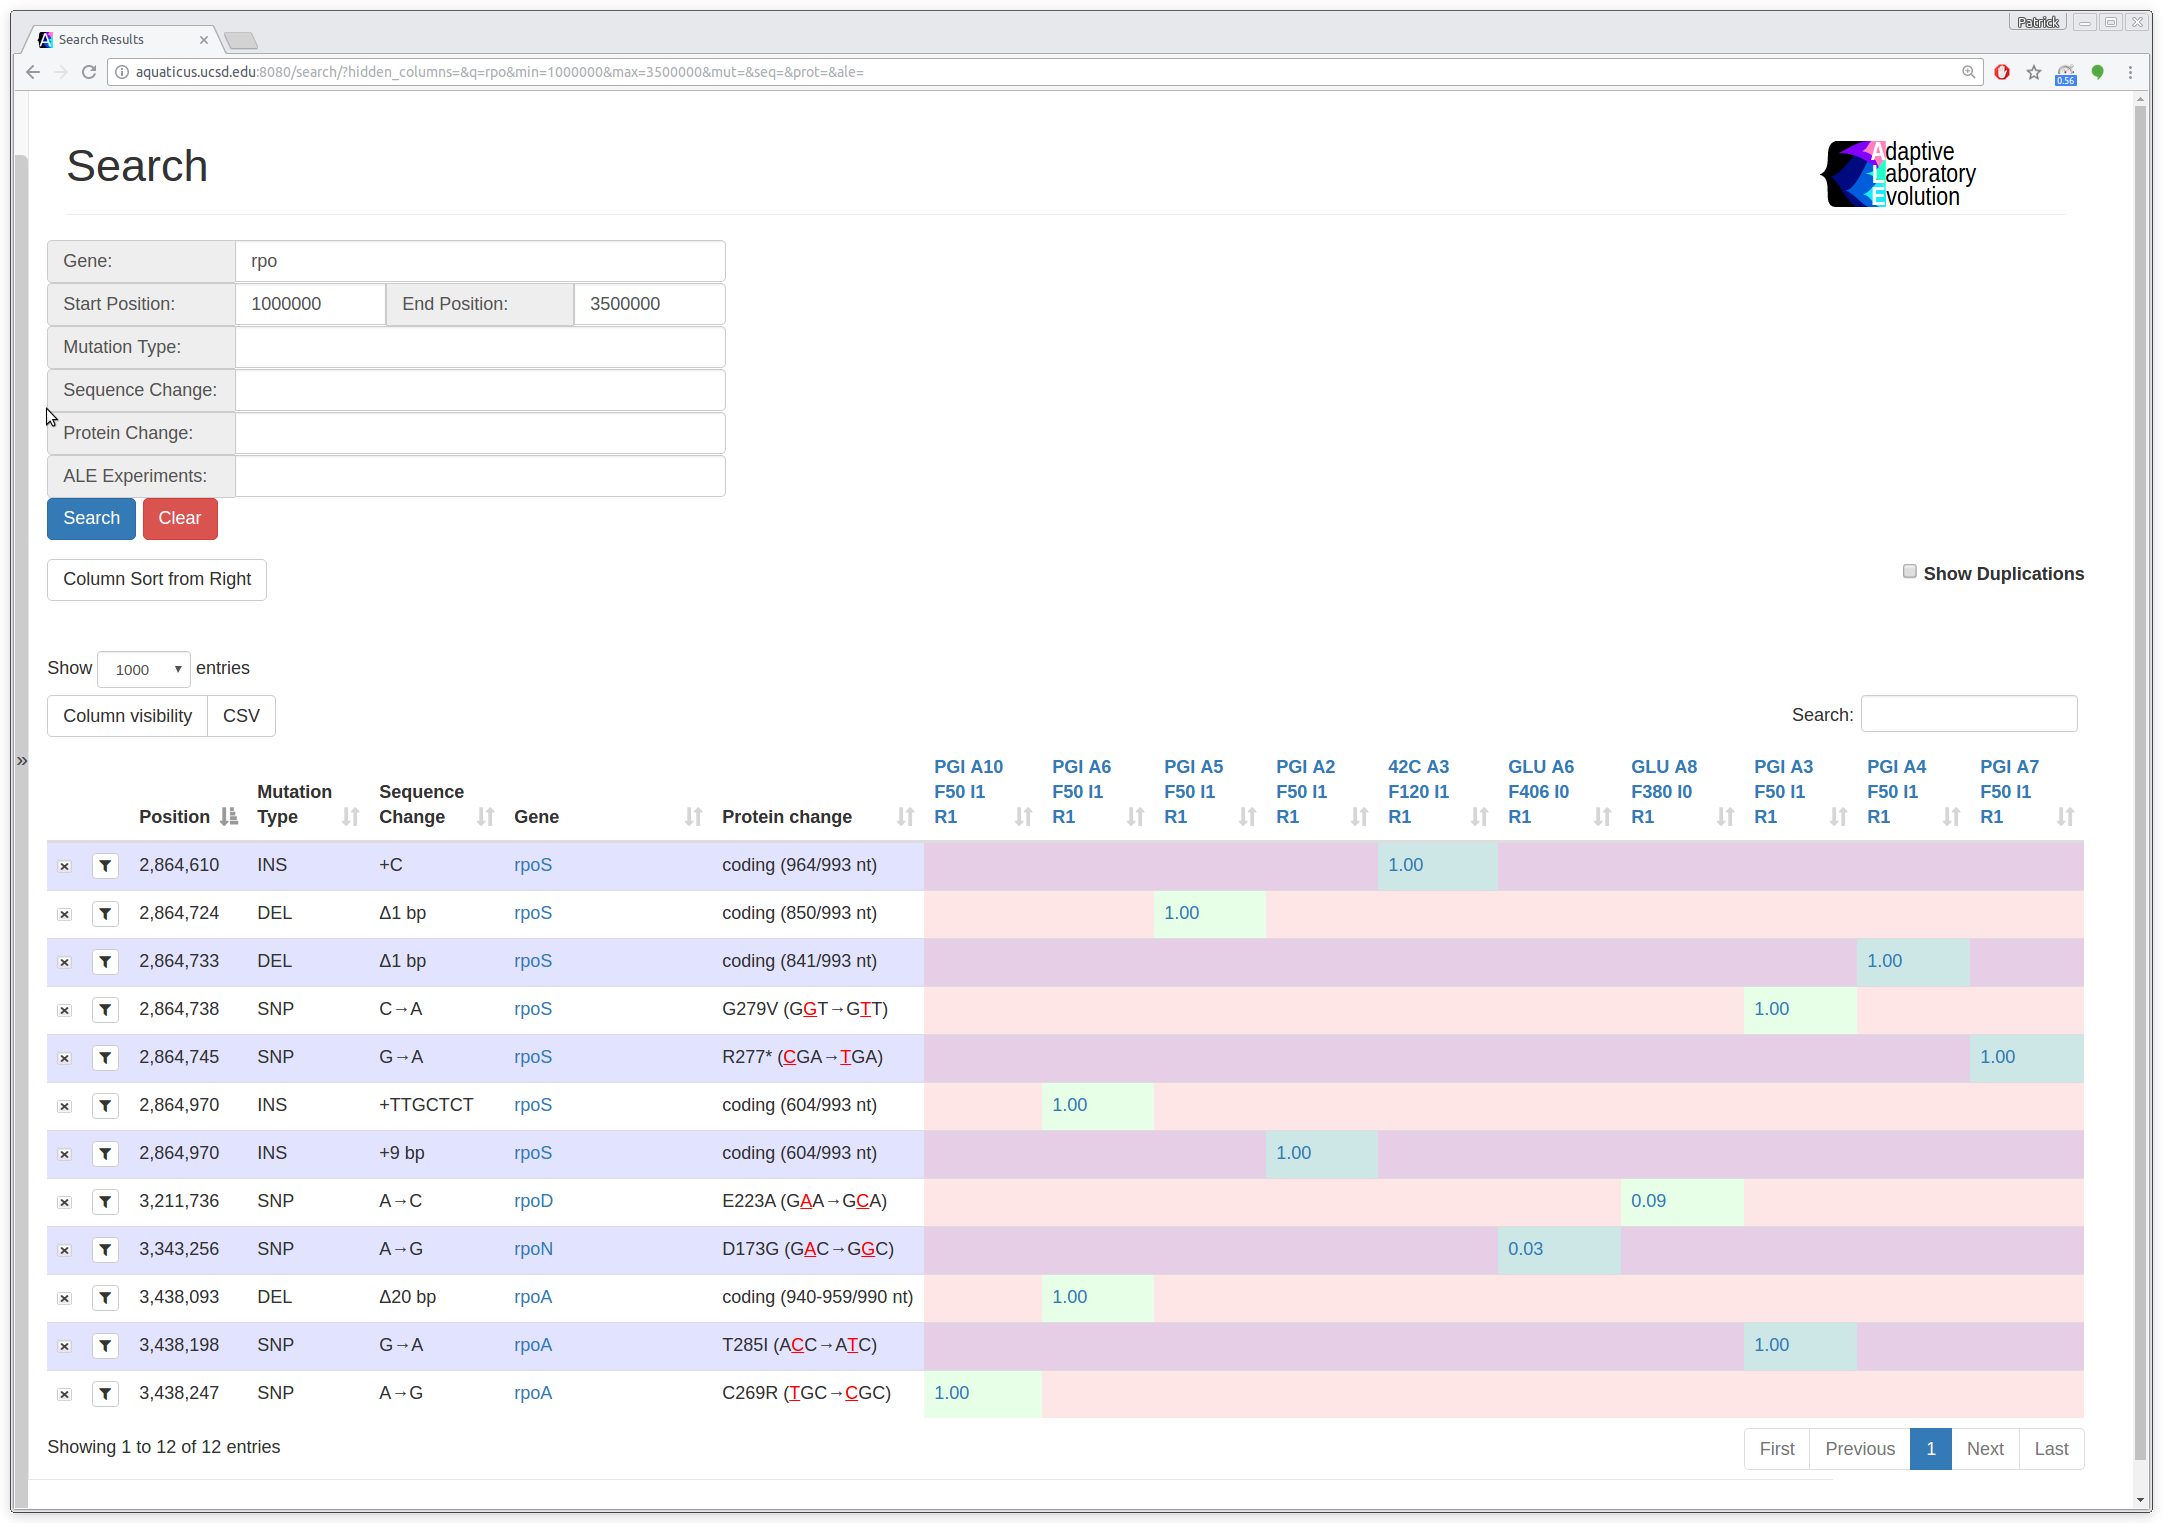
\includegraphics[width=0.9\textwidth]{search_page.png}
  \caption[A screenshot of the mutation search page and search result's mutation report for the instance of ALE Analytics used to accomplish the analysis contained within this thesis.]{ The search functionality uses as mutation query parameters the \textit{gene}, \textit{start} and \textit{end positions}, \textit{mutation type}, \textit{sequence change}, \textit{protein change} and ALE experiment of mutations.}
  \label{fig:search_page}
\end{figure}
%It is likely that users will want to leverage experiment analysis specific to the context of their experiments. The ALE Analytics experiment export feature, which enables the extraction of mutation data from one or more experiments as a comma separated value file, allows for end users to implement custom analysis protocols in pursuit of their individual hypothesis and leverage them on the consolidated ALE experiment data.
Experimentalists invent many different data mining protocols for exploring the data housed within the mutation database. It would not be practical to implement all of these protocols into ALE Analytics, though it is clear that experimentalists should have the ability to easily extract data sets from the mutation database for their own investigations. The ALE experiment export feature was implemented to support this case; it enables users to extract all mutations from one or more ALE experiments. Experimentalists and investigators are then free to implement data mining protocols of their own design on the ALE data. Figure \ref{fig:all_muts_topo} presents histograms generated using the export feature and external tools to explore the position and frequency of mutations affecting the genomes of the ALE experiments used in the analysis contained within this thesis.
\begin{figure}[H]
  \centering
  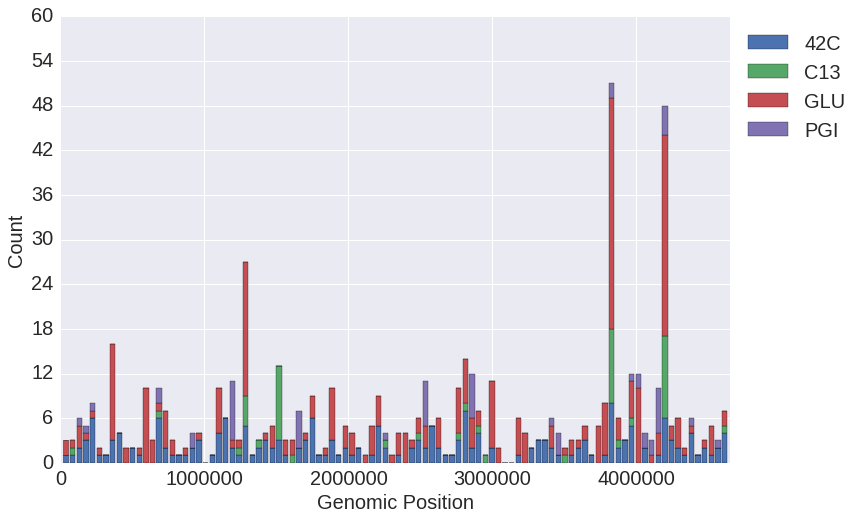
\includegraphics[width=0.9\textwidth]{all_muts_topo.png}
  \caption[A histogram of all mutation positions contained within the instance of ALE Analytics used to accomplish the analysis contained within this thesis.]{ Mutation positions are divided into 100 bins and the results of the different ALE experiments involved are stacked to visualize the cumulative mutation frequency within a genomic region.}
  \label{fig:all_muts_topo}
\end{figure}
% \begin{figure}[H]
%   \caption{A histogram of all SNPs of evaluation ALE experiments.}
%   \centering
%   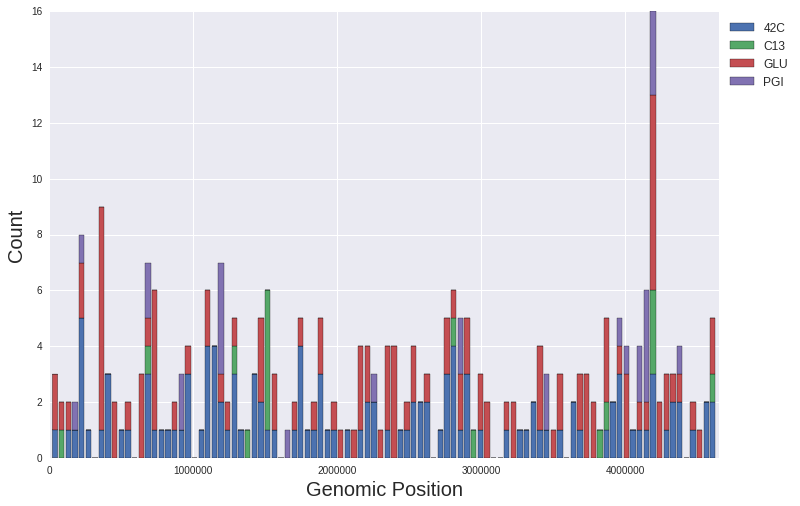
\includegraphics[width=0.9\textwidth]{all_snps_topo.png}
%   \label{fig:all_snps_topo}
% \end{figure}
% \begin{figure}[H]
%   \caption{A histogram of all mobile insertion elements of evaluation ALE experiments.}
%   \centering
%   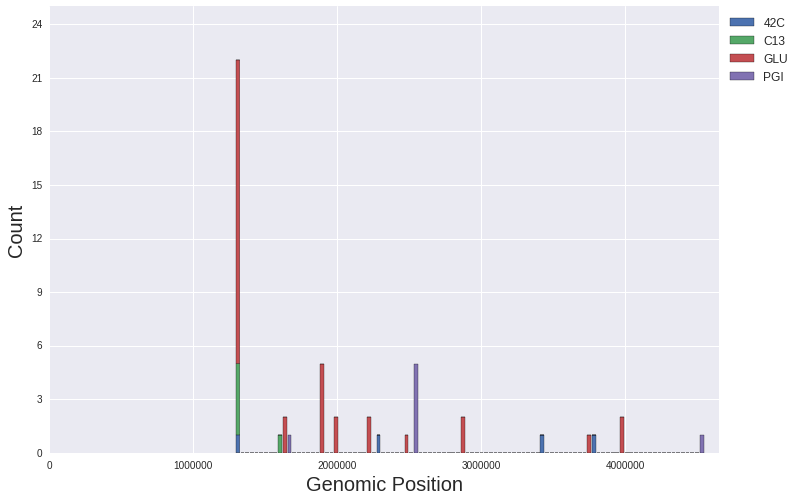
\includegraphics[width=0.9\textwidth]{all_mobs_topo.png}
%   \label{fig:all_mobs_topo}
% \end{figure}
% \begin{figure}[H]
%   \caption{A histogram of all small insertions of evaluation ALE experiments.}
%   \centering
%   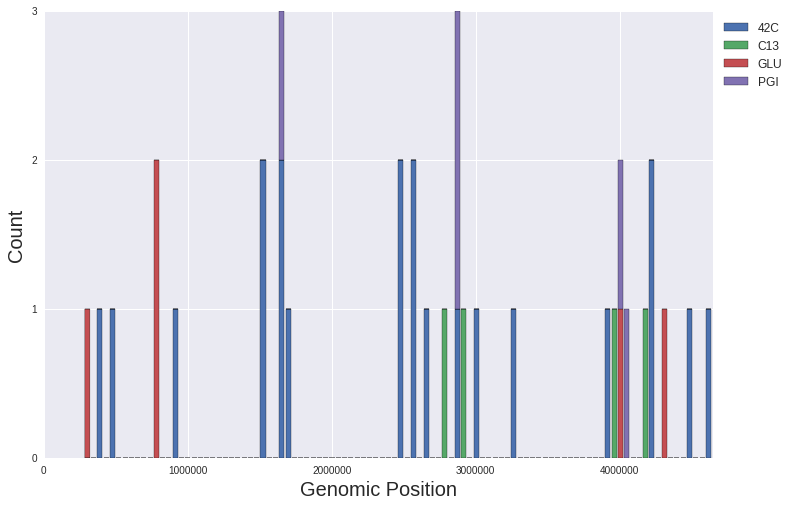
\includegraphics[width=0.9\textwidth]{all_ins_topo.png}
%   \label{fig:all_ins_topo}
% \end{figure}
% \begin{figure}[H]
%   \caption{A histogram of all deletions of evaluation ALE experiments.}
%   \centering
%   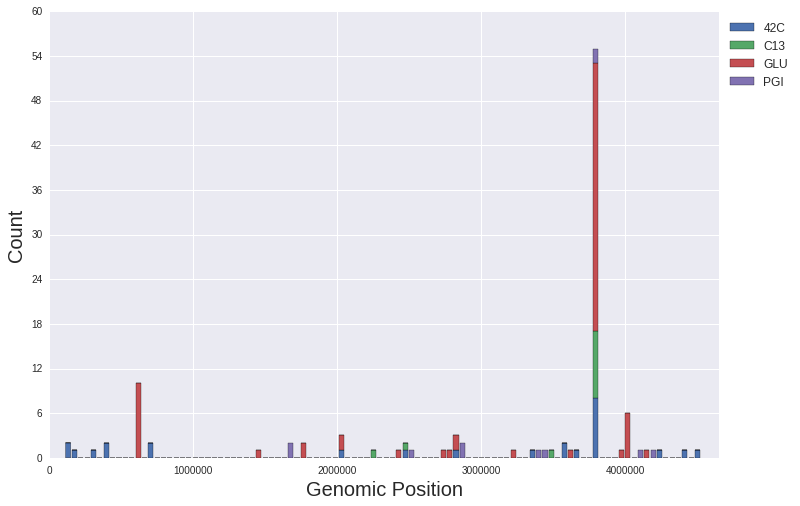
\includegraphics[width=0.9\textwidth]{all_dels_topo.png}
%   \label{fig:all_dels_topo}
% \end{figure}

% This type of investigation enables users to quickly where mutation hotspots exists. For instance, in \ref{fig:all_muts_topo}, we can see there exists a mutation hotspot involving all ALE experiments at approximately 4.4MB. 

\clearpage
I would like to acknowledge Dennis Gosting for his work in implementing the current version of the majority of the user features described in this section.

I would like to acknowledge Anand Sastry for his work in implementing external data mining protocols to which I leveraged in generating the histogram figure include in this thesis of all mutations positions for the ALE experiments used in the evaluation of the automated analysis.
\clearpage
\section{ALE Analytics Platform Deployment Overview}
A production version of ALE Analytics has been deployed since August 2015 and has therefore been a live solution for more than a year to the ALE big data to knowledge challenges of the SBRG and the Novo Nordisk Center for Biosustainability of Lyngby, Denmark. Since this deployment, the ALE mutation database and the ALE Analytics platform have seen a dramatic increase in usage and ALE experiment data. Effort was devoted into designing a deployment environment using industry standard technologies and methodologies that would enable the platform's data to be secure and have redundant copies on external secure file servers.

\begin{figure}[H]
  \centering
  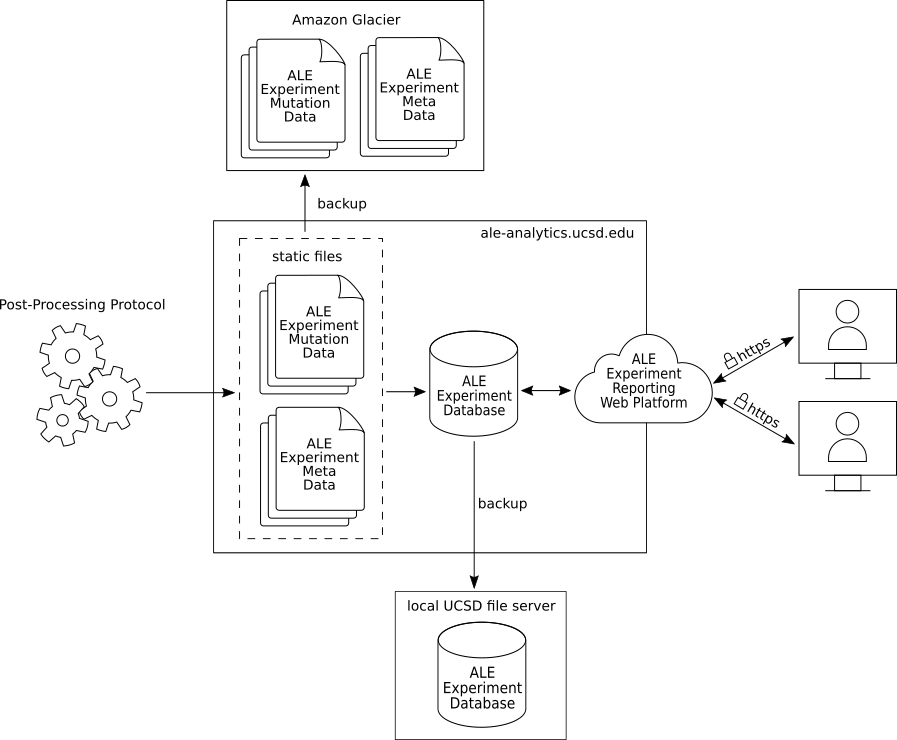
\includegraphics[width=0.9\textwidth]{deployment_diagram.png}
  \caption{An illustration of the deployment environment for the ALE mutation database and ALE Analytics platform that describes important data security and redundancy measures.}
  \label{fig:deployment_diagram}
\end{figure}

The platform makes use of the \textit{Linux}, \textit{Django} \cite{django} and \textit{Nginx} \cite{nginx} web application technology stack to deploy ALE Analytics from a dedicated server hosted by the San Diego Supercomputer Center. The static files that are used in populating the ALE mutation database and contain mutation reports referenced by ALE Analytics analyses are hosted on the same server and have backups on external servers through the Amazon Glacier file storage service (Amazon Web Services, Seattle, WA). The Amazon Glacier service is used due to the cumulative static file storage footprint of approximately 1.8 terabytes and this service's competitive storage costs. The ALE mutation database has a small enough storage footprint that it can have backups on a file server internal to UCSD and accessible only to SBRG members and IT staff. All reads used in generating the static files are also stored on the same internal file server. User access to the ALE Analytics data is controlled through a user account management system provided by the Django and Nginx technologies and all browsing traffic is encrypted via HTTPS protocol.
\chapter{Conclusion}
%Review how this project is currently enabling Big Data to Knowledge.
The SBRG's ALE experiment automation has scaled the rate of experiment execution and data generation to the point that data post-processing, consolidation, reporting and common analysis have become a primary bottleneck in interpreting results. The SBRG's ALE methodologies therefore require a big data to knowledge solution that automates these bottlenecks to match the rate of high-throughput ALE experimentation. We have developed a software system that addresses each challenge that defines the big data to knowledge solution. To address quality control and mutation data formatting challenges, we investigate and establish a post-processing software pipeline. To address the challenge of high-throughput ALE experiment data consolidation, data reporting and common analysis, we implement the ALE Analytics software platform. The automated common analysis are evaluated against currently published ALE experiment key mutation results and show that they are precise, maintain high recall and can be expanded upon for more comprehensive predictions. We have additionally developed the ALE Analytics reporting and analysis platform as a web application to address the challenge of accessible experiment reporting. We go beyond these challenges and their solutions and have implemented features that leverage the consolidated data to find key mutations shared among all ALE experiments. Finally, we have shown how ALE Analytics has implemented beyond the core challenge solving features to culminate in a platform that supports the multitude of services experimentalists currently need to execute their ALE experiment analysis.

Quality control protocols and tools have been investigated and combined into an ALE post-processing protocol. This protocol provides stage-dependent feedback that is crucial for all those involved in the ALE sample preparation and processing, as it informs them of their work's quality and better enables root-causing of quality issues.

Our system's automated common ALE experiment mutation analysis has been shown to be precise and maintain high recall in finding key mutations of published data sets. Of the published ALE experiments, an average recall of 89.6\% and an average precision of 71.2\% is achieved when excluding hypermutators. The automated key mutation analysis additionally identified key mutations in genes \textit{wecA} and \textit{yjiT} that were not included in the published material yet were aligned with their published key mutation protocols. Our automated key mutation analysis may lead to better result accuracy due to less potential for human error and variation in protocol between experimentalists.

The consolidation of ALE experiment data offers an opportunity for cross-experiment analysis. ALE Analytics has leveraged this opportunity with the implementation of the shared key mutations feature, which generates reports identifying genomic regions affected by key mutations in multiple ALE experiments. The ALE experiments used in evaluating the automated key mutation features manifests five of these shared key mutation genomic regions: \textit{rph}, \textit{hns-tdk}, \textit{rpoB}, \textit{rpoC} and \textit{pykF}. The \textit{rph} genomic region is mutated by key mutations in all provided ALE experiments and is proposed to be an adaptation for a defect that exists with the starting strain of these experiments \cite{Conrad2009}. The \textit{hns-tdk}, \textit{rpoB} and \textit{rpoC} genomic regions are each affected by key mutations in at least two ALE experiments and are proposed to be adaptive adjustments to global transcriptional regulation that benefit host growth rates \cite{Kobayashi01011990, AYERS1989749, Cheng2014, Wang1445}. Key mutations affect the \textit{pykF} gene in two ALE experiments and are speculated to contribute to the hosts growth rate by enabling a larger rate of glucose uptake through the disabling of a phosphenopyruvate metabolic process \cite{Woods13062006, 10.1371/journal.pgen.1001164, Blank25022014}. Disrupting \textit{pykF} could render a fitness benefit in conjunction with the glucose rich media used in these experiments.

The work of this thesis does not stop at proposing and prototyping a possible big data to knowledge solution, but has in fact been deployed as a tool for ALE experimentalists at the System Biology Research Group and the Novo Nordisk Center for Biosustainability of Lyngby, Denmark, since August 2015. The current deployment leverages an industrial strength technology stack and production environment of Django, Nginx and Linux on a dedicated server hosted by the San Diego Supercomputer Center and strives to ensure security through user accounts and HTTPS encrypted browsing.% At this time, the tools and analysis of ALE Analytics have significantly contributed to the results of one metabolic research project whose results are currently in the process of being accepted for publication \cite{l-serine}.

With this thesis' work, it is clear that the SBRG's ALE operations can now overcome its consolidation and reporting bottlenecks. This is exemplified by the current count of 42 ALE experiments, 325 ALEs and 14,765 observed mutations currently housed within the ALE experiment and mutation database, where each mutation is represent in an ALE experiment's mutation reports. The SBRG's ALE operations should in fact increase the number of samples per ALE experiment analysis sample set to better enable the automated analysis in predicting key mutations by effectively increasing the resolution of mutations in an evolution. Population samples, which reveal both consensus and population mutations, can additionally be included at higher frequencies in analysis sample sets to enable the exploration of population evolution dynamics. This research has yet to be thoroughly examined within high-throughput ALE experiments due to the effort necessary in the curation of the magnitude of mutations involved with population samples.

ALE Analytics automated key mutations analysis could be enhanced by including ALE sample growth rate data and by investigating perturbations in the context of functionally related gene groups. ALE sample growth rate data, which describes the growth rate of samples during the progression of an ALE, can be used to automate the identification of mutations correlated with growth rate spikes. Mutations uniquely affecting genomic regions can be considered significant if they perturb a functionally related gene group which hosts additional mutations. Using these new data types and contexts, the automated key mutation analysis can therefore be expanded to consider multiple categories of evidence for significance.

Going forward, the ALE experiment mutation database presents an amazing opportunity for research into mutational trends across all ALE experiments available to the SBRG. Already, data mining protocol have made use of ALE Analytic's experiment export feature and have been used to characterize the general topology of mutations across the \textit{E. coli} K-12 MG1655 genome from multiple ALE experiments. As ALE Analytics continues to integrate new ALE experiments, current and new data mining protocols can scan the ALE experiment mutation database in the hope of identifying previously unseen trends.

%% APPENDIX
\appendix

%% END MATTER
% \printindex %% Uncomment to display the index
% \nocite{}  %% Put any references that you want to include in the bib 
%               but haven't cited in the braces.
\bibliographystyle{plain}  %% This is just my personal favorite style. 
%                              There are many others.
%\setlength{\bibleftmargin}{0.25in}  % indent each item
%\setlength{\bibindent}{-\bibleftmargin}  % unindent the first line
%\def\baselinestretch{1.0}  % force single spacing
%\setlength{\bibitemsep}{0.16in}  % add extra space between items
\bibliography{template}  %% This looks for the bibliography in template.bib 
%                          which should be formatted as a bibtex file.
%                          and needs to be separately compiled into a bbl file.
\end{document}

